\documentclass[11pt,aspectratio=169]{beamer}
% Deliberately simple: default theme, no Metropolis (matches the primer deck).
\usetheme{default}
\usecolortheme{dove}
\usefonttheme{serif}
\setbeamertemplate{navigation symbols}{}
\setbeamertemplate{footline}{}
\setbeamertemplate{itemize items}[circle]

\usepackage{amsmath,amssymb}
\usepackage{booktabs}
\usepackage{graphicx}
\usepackage{xcolor}
\usepackage[most]{tcolorbox}
\usepackage{minted}
\usemintedstyle{friendly}                 % colorful pygments theme
\setminted{fontsize=\scriptsize,breaklines,autogobble,tabsize=2,escapeinside=||}
\setminted[cpp]{fontsize=\scriptsize}
\setminted[python]{fontsize=\scriptsize}

\graphicspath{{figs/}{../paper/figures/}{../figs/}}

\definecolor{key}{rgb}{0.10,0.35,0.65}
\newcommand{\bhat}{\hat{\mathbf{b}}}
\setbeamercolor{frametitle}{fg=key}
% small manual footnote (no marker collisions)
\newcommand{\notefoot}[1]{\vfill{\footnotesize #1\par}}

% ------------------------------------------------------------
% Helper for the interleaved RED speaker-notes frames.
% Every notes frame is allowframebreaks so long notes never overflow.
% ------------------------------------------------------------

\title{A Native Spin-Polarized Neutron Source in OpenMC}
\subtitle{From \texttt{TokamakSource} to a 3-D Equilibrium \texttt{StellaratorSource}}
\author{Thaddaeus Kiker}
\date{\today}

\begin{document}
\frame{\titlepage}

% ============================================================
\begin{frame}{Miscellaneous Updates}
\begin{itemize}
\item Scheduling a meeting with Dr.\ Elizabeth Paul (Columbia) to discuss quasi-symmetry
      and stellarator optimization, and how her equilibrium/QS expertise could inform the
      QUASR device selection and equilibrium inputs feeding this source.
\item My apartment building caught on fire yesterday (photos follow).
\end{itemize}
\end{frame}

\begin{frame}[allowframebreaks]{Notes --- Miscellaneous Updates}
{\color{red}\footnotesize
\begin{itemize}
\item This is the housekeeping slide before the technical content. Two bullets: (1) a
      planned meeting with Elizabeth Paul (Columbia stellarator-optimization / quasi-symmetry
      theorist) and (2) a personal note that my apartment building caught on fire, with two
      photos on the following slides.
\item Why Paul is relevant: she works on quasi-symmetry and stellarator coil/boundary
      optimization. The predictor half of this project leans on quasi-symmetry (QA/QH) device
      classes drawn from the QUASR database, so a conversation with her is a natural way to
      pressure-test the geometry/equilibrium side of the work.
\item Keep this slide to ~15 seconds. It is not technical; do not let it eat into the physics.
\item Likely follow-up (Ethan): ``are you OK / do you need to reschedule?'' --- crisp answer:
      yes, the work is done and reproducible; the photos are just context for why I might be
      slower on email this week.
\end{itemize}
}
\end{frame}

\begin{frame}{Miscellaneous Updates}
\centering
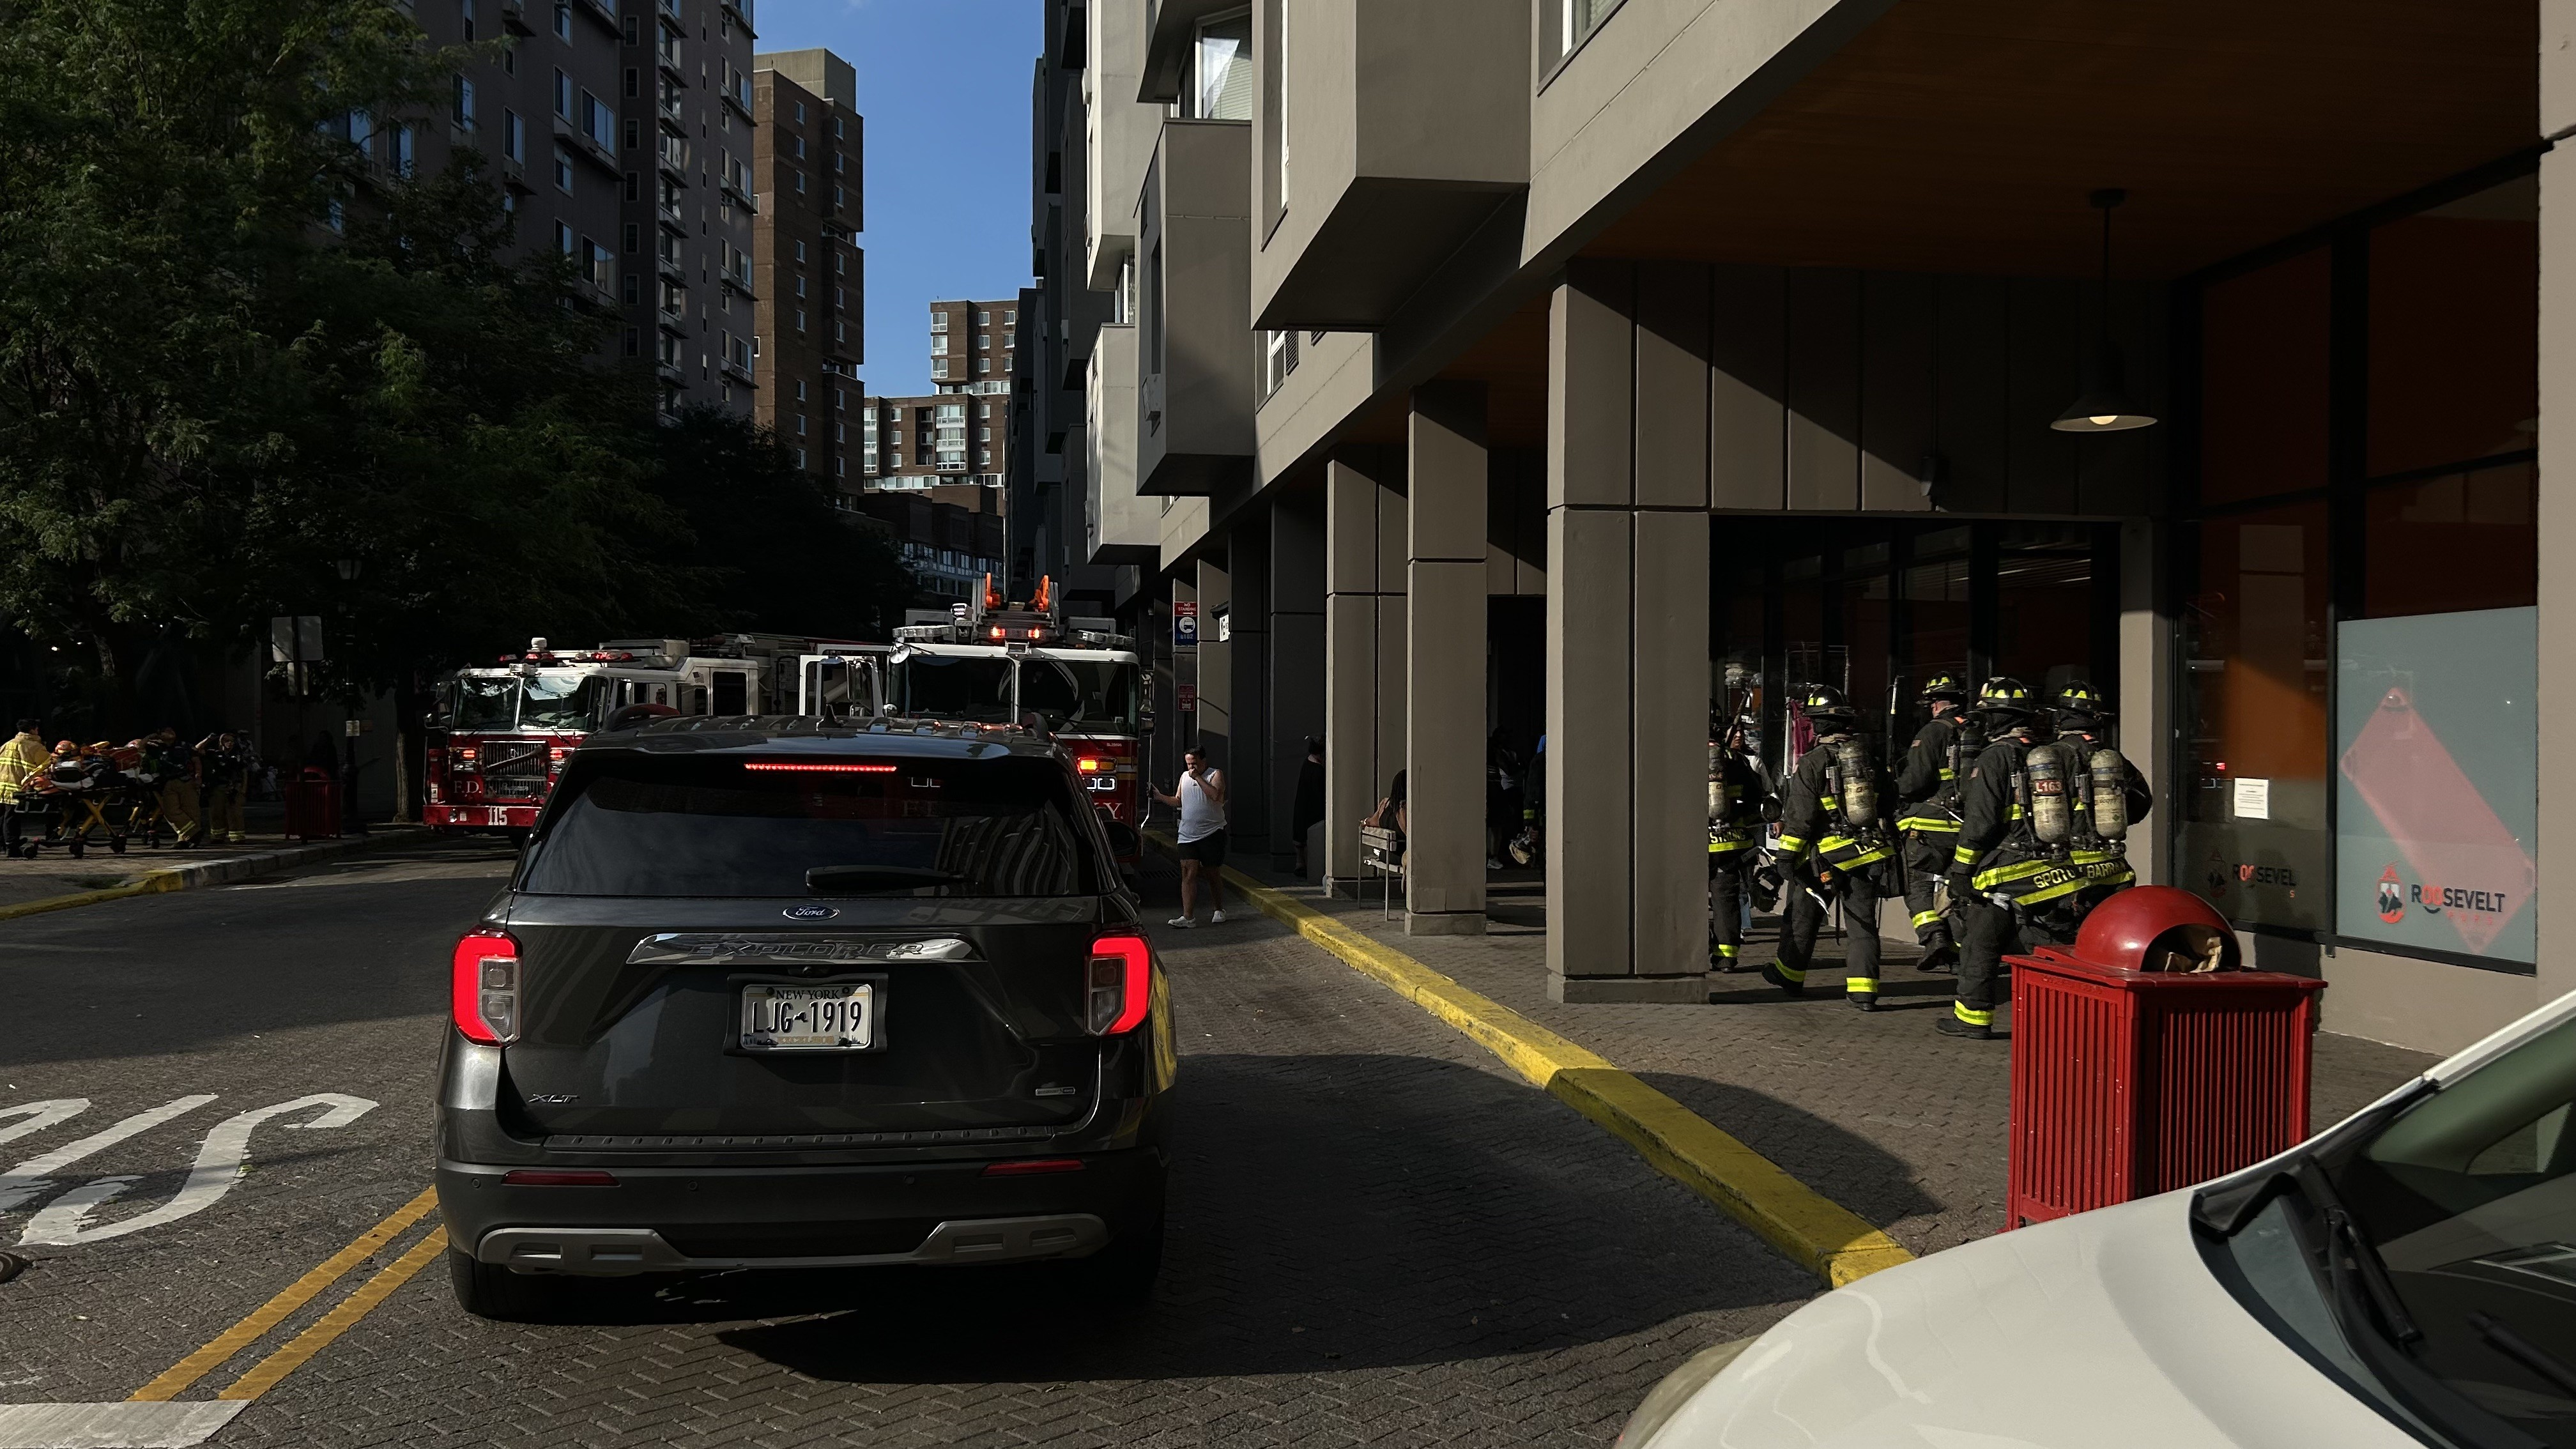
\includegraphics[width=0.92\linewidth]{misc_fire1.jpg}
\end{frame}

\begin{frame}{Miscellaneous Updates}
\centering
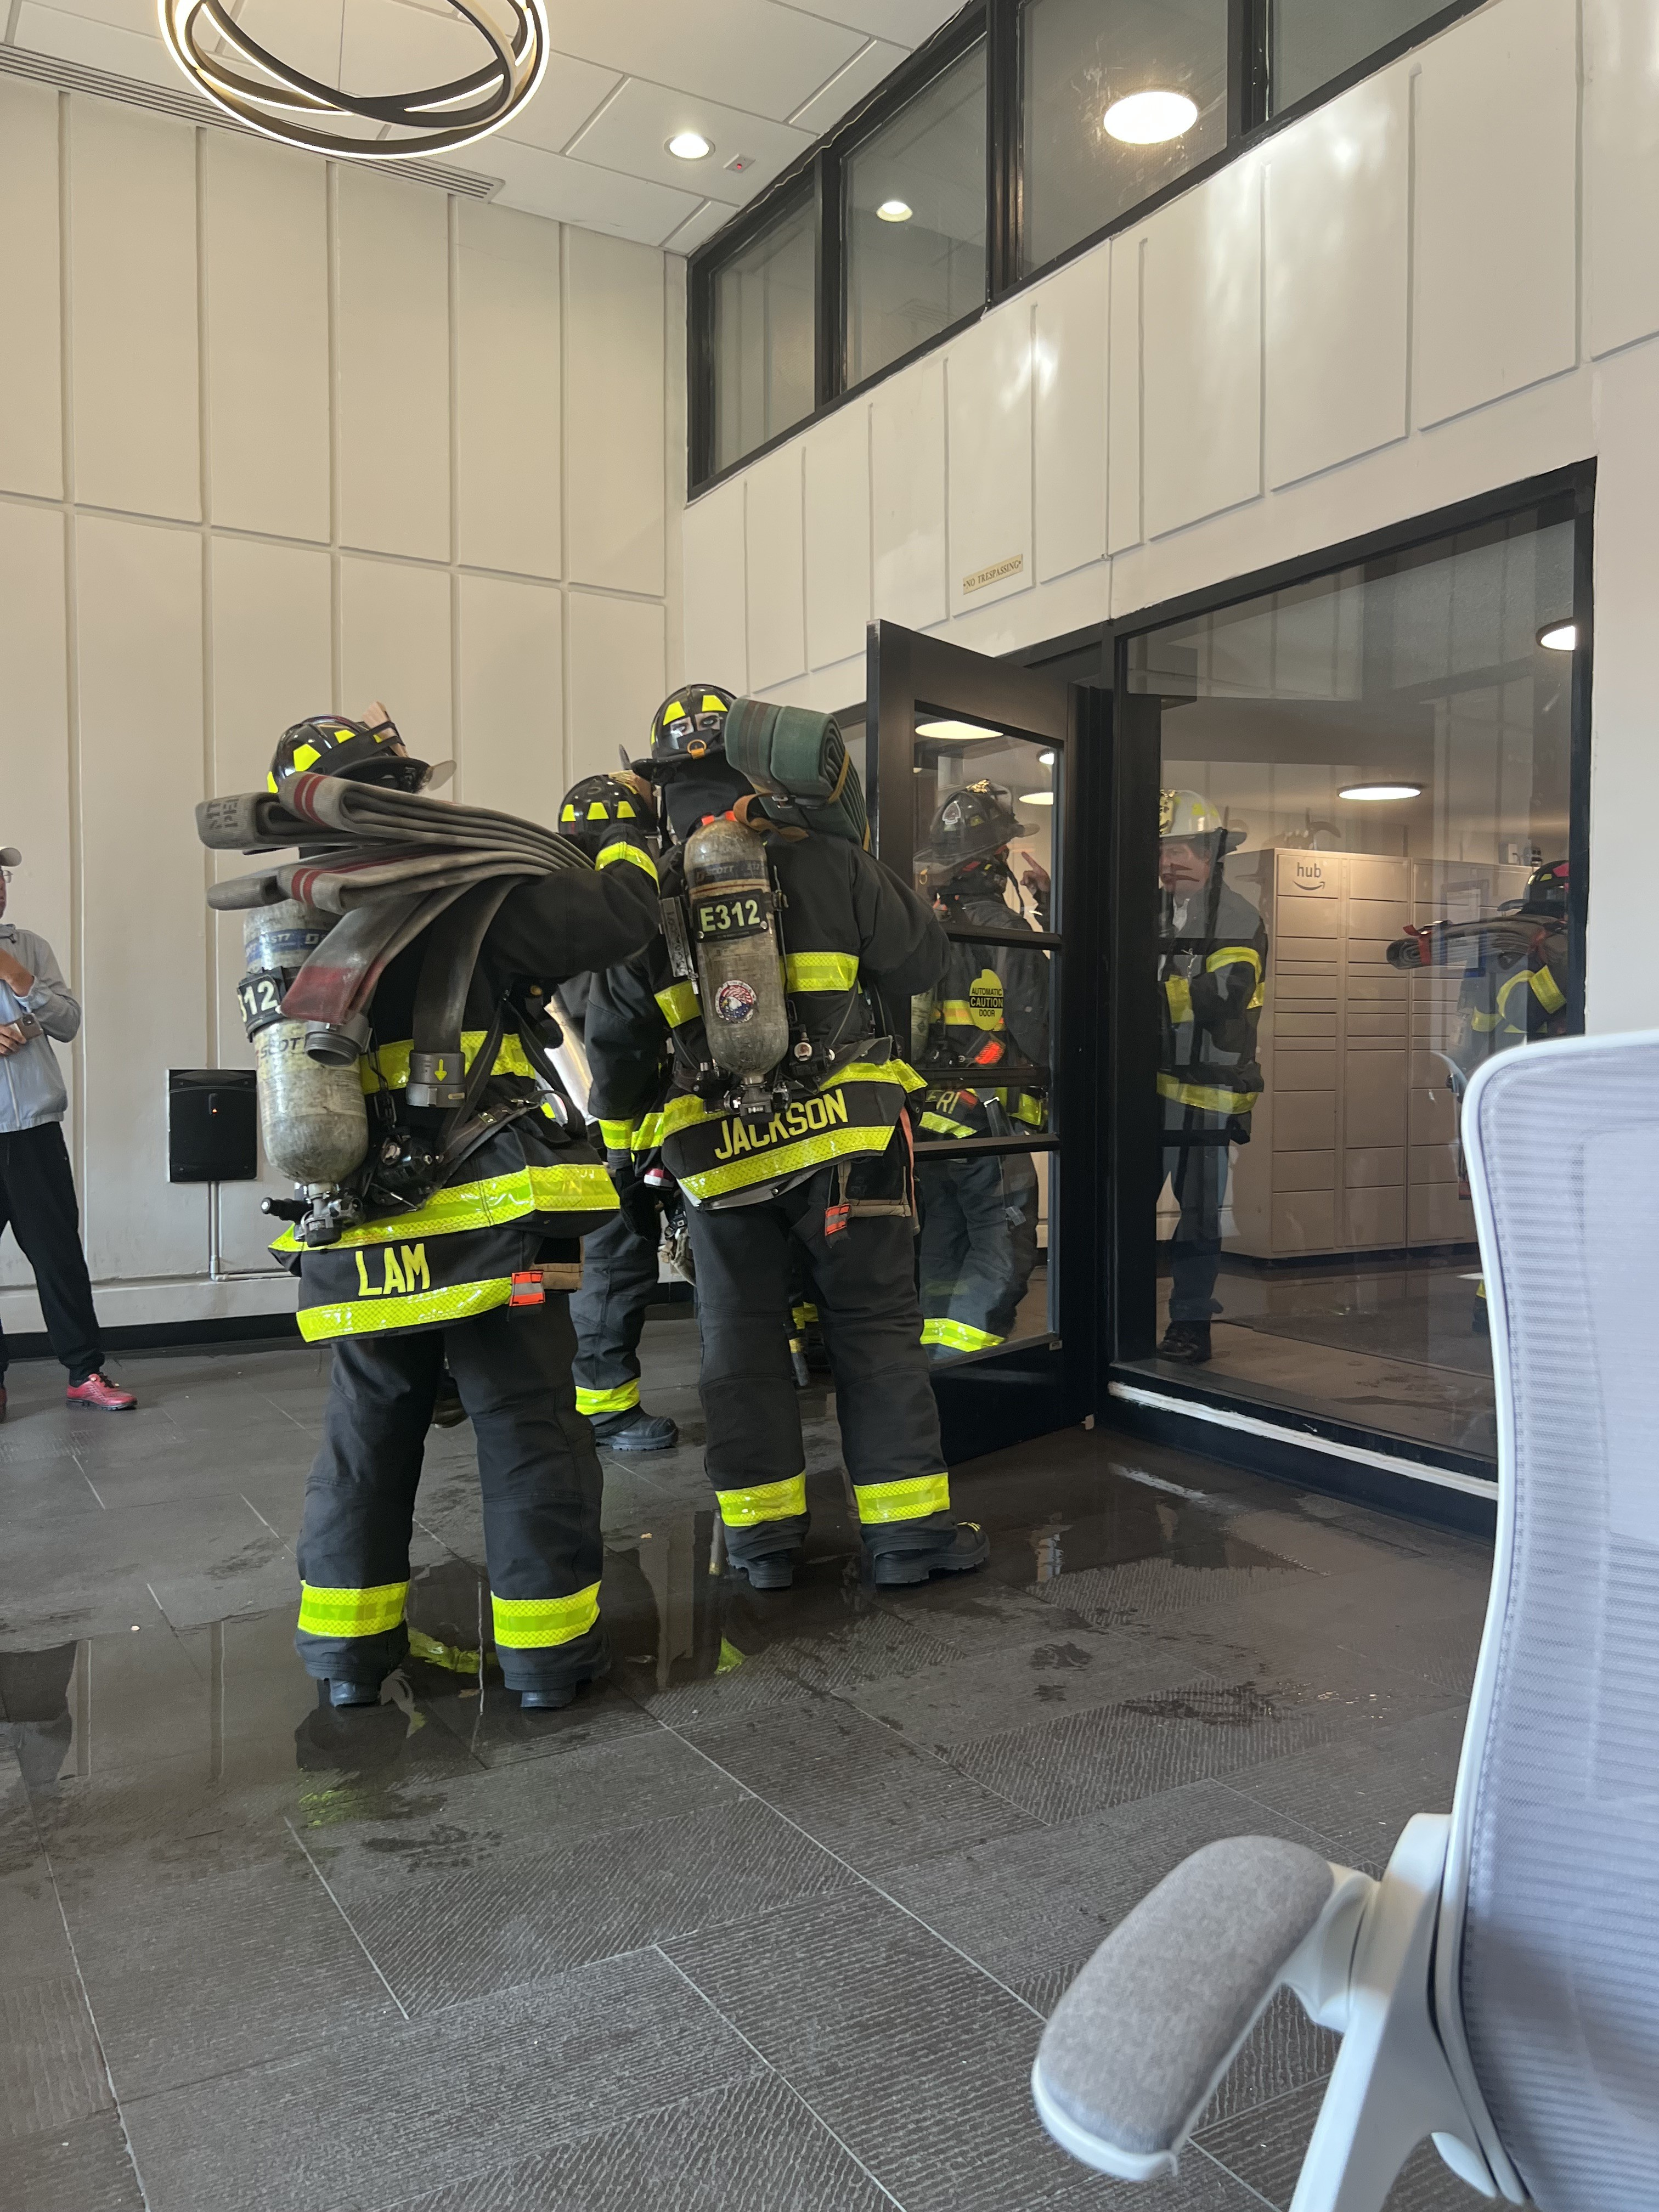
\includegraphics[height=0.84\textheight]{misc_fire2.jpg}
\end{frame}

% ============================================================
\begin{frame}{What I Built This Week}
\begin{itemize}
\item A native OpenMC C++ \texttt{Source} subclass that samples spin-polarized D--T
      neutron emission in the local field frame, driven by a real 3-D equilibrium flux
      map (DESC/VMEC).\footnote{\scriptsize A precomputed, tabulated OpenMC tokamak
      neutron source also exists (Bae et al., Nucl.\ Fusion 65, 086051, 2025); it bakes
      the emission into a fixed sampled distribution rather than generating it natively on
      the fly, so it cannot carry the local-field-dependent polarized direction.}
\item Built on the \texttt{TokamakSource} pattern (PR \#3999): the same rejection-free CDF
      cascade and native-\texttt{Source} plumbing.
\item Adds polarized emission about $\bhat$, real equilibrium geometry with $\sqrt{g}$
      weighting, and genuine three-dimensionality.
\item Verified against analytic theory, cross-checked on real QUASR geometry, and run
      end-to-end through a conformal multi-material blanket.
\end{itemize}
\end{frame}

\begin{frame}[allowframebreaks]{Notes --- What I Built This Week}
{\color{red}\footnotesize
\begin{itemize}
\item This is the thesis slide: one native OpenMC C++ \texttt{Source} subclass that samples
      (a) a birth position from a real 3-D equilibrium and (b) a spin-polarized emission
      direction about the local magnetic field $\bhat$. ``Native'' means the sampling runs
      inside the transport loop, per history, in C++, not replayed from a precomputed table.
\item ``Local field frame'' matters: the anisotropy is defined relative to $\bhat$ at the
      birth point, and $\bhat$ varies in space. A tabulated point-cloud source cannot carry a
      space-varying polarization axis --- that is the whole reason a native sampler is needed.
\item The footnote is the Bae et al.\ 2025 (Nucl.\ Fusion 65, 086051) framing. Bae published a
      precomputed, tabulated polarized tokamak source in OpenMC first. Do NOT claim ``first
      polarized source in OpenMC'' --- Bae has that. DO claim ``first \emph{native / general /
      on-the-fly} polarized source,'' i.e.\ one that generates position+polarized direction
      inside the transport loop from a real equilibrium, so $\bhat$ can vary in space. One-liner:
      ``Bae replays a frozen tokamak source; we generate a local-field-aware polarized source on
      the fly, for any equilibrium.'' (QA\_RESEARCH Q38.)
\item ``Built on the TokamakSource pattern (PR \#3999)'': Ethan Peterson's TokamakSource is the
      template. We reuse its \emph{plumbing} (a \texttt{public openmc::Source} subclass, a
      constructor taking a \texttt{pugi::xml\_node}, \texttt{SourceSite sample(uint64\_t*) const
      override}, the Python \texttt{SourceBase} subclass, XML round-trip) and its
      \emph{rejection-free CDF cascade} idea for sampling position. We do NOT reuse its position
      \emph{math} (Miller geometry), because a stellarator has no closed-form boundary.
\item ``$\sqrt{g}$ weighting'' = the metric Jacobian of the flux coordinates; it makes the
      birth-position density a true \emph{volumetric} source rather than uniform-in-coordinate.
      Explained in detail on the position-code slide.
\item ``Genuinely three-dimensional'': the equilibrium is non-axisymmetric $(\rho,\theta,\zeta)$;
      $\bhat$ is a full 3-D gridded field, not $\hat\varphi$.
\item Last bullet is the validation ladder, which the rest of the talk walks: (1) sampler exact
      vs analytic (Tier 1), (2) free-streaming recovers Schwartz on the box torus and on real
      QUASR geometry, (3) end-to-end transport through a conformal DAGMC blanket with scattering.
\item HOW/WHERE: the two C++ translation units live under
      \texttt{spf\_prototype/native\_spf/} (\texttt{source.cpp} = SPF-patched Tokamak;
      \texttt{stellarator\_source.cpp} = the new class). Validated Python oracle is
      \texttt{ConformalStellaratorSampler}; RNG mirror is \texttt{spf\_mirror.py}.
\item Likely follow-up (Ethan): ``how is this different from your source vs mine?'' --- crisp:
      same Source pattern; we add a polarized-direction hook (upstreamable into TokamakSource)
      plus a sibling StellaratorSource for real 3-D equilibria with grid-field $\bhat$
      (QA\_RESEARCH Q40).
\end{itemize}
}
\end{frame}

% ============================================================
\begin{frame}{Lineage}
\begin{itemize}
\item \texttt{source.cpp.orig}: your \texttt{TokamakSource} (PR \#3999). Parametric
      Miller geometry, rejection-free cascade in $(r/a,\alpha,\phi)$, isotropic emission.
\item \texttt{source.cpp}: my SPF patch to that class. Added the polarized-direction
      machinery (\texttt{sample\_polarized\_direction}, \texttt{field\_model}, the
      $(a,b,c)\!\to\!w_\perp,w_\parallel$ mixture).
\item \texttt{stellarator\_source.cpp}: the new class. Same direction sampler, but geometry
      comes from a real equilibrium flux map with $\sqrt{g}$ weighting and a gridded 3-D
      $\bhat$.
\end{itemize}
\notefoot{$\dagger$~Note: my prototype emits monoenergetic 14.06\,MeV, whereas your
\texttt{TokamakSource} supports per-$r$ energy spectra.}
\end{frame}

\begin{frame}[allowframebreaks]{Notes --- Lineage}
{\color{red}\footnotesize
\begin{itemize}
\item This slide shows three files as an evolutionary chain, so Ethan sees exactly what was
      reused vs\ rewritten from his PR \#3999.
\item \texttt{source.cpp.orig} = an unmodified copy of Peterson's TokamakSource: parametric
      Miller equilibrium $(R_0,a,\kappa,\delta,\Delta)$, a rejection-free CDF cascade in
      $(r/a,\alpha,\phi)$, and isotropic (unpolarized) emission with per-flux-surface energy
      spectra. This is the baseline.
\item \texttt{source.cpp} = my \emph{patch} to that same class. I added an optional
      \texttt{<polarization>} node (absent $\Rightarrow$ unchanged isotropic behavior, so it is
      backward-compatible), the direction sampler \texttt{sample\_polarized\_direction}, a
      \texttt{field\_model} selector, and the $(a,b,c)\!\to\!(w_\perp,w_\parallel)$ mixture
      algebra. This demonstrates the polarized hook is upstreamable straight into TokamakSource.
\item \texttt{stellarator\_source.cpp} = the genuinely new translation unit. It shares the
      \emph{direction} sampler verbatim (diff-confirmed identical code) but replaces the
      \emph{position} machinery: geometry now comes from a real gridded equilibrium flux map
      with $\sqrt{g}$ weighting, and $\bhat$ comes from the same 3-D grid $(B_R,B_\phi,B_Z)$.
\item Key mental model (QA\_RESEARCH Q1/Q2): ``two position models, one direction model.''
      Reused verbatim = the SPF direction sampler, the per-shape inverse-CDF roots
      \texttt{spf\_costheta\_perp/par}, and the $(a,b,c)\!\to\!w_\perp/w_\parallel/P_\perp$
      block. Reused pattern = the Source subclass plumbing. Rewritten = the
      \texttt{spf\_fluxmap\_v1} reader, the CDF cascade \texttt{build\_cdf\_cascade}, trilinear
      interp with $\theta/\zeta$ period wrap, and the $\bhat$-from-grid path.
\item The footnote ($\dagger$) is an honest limitation stated up front: my prototype emits
      monoenergetic 14.06\,MeV, while TokamakSource supports per-$r$ (per-flux-surface) Ballabio
      energy spectra. Why it is fine: energy is decoupled from the polarized \emph{angular}
      distribution to leading order, and the steering/NWL verification is energy-independent. A
      per-$r$ spectrum is a drop-in extension --- the XML already loops \texttt{<energy>}
      (QA\_RESEARCH Q20/Q42).
\item Likely follow-up (Ethan): ``why a new class instead of just extending TokamakSource?'' ---
      crisp: TokamakSource generates positions from an analytic parametric equilibrium; a
      stellarator has no closed-form boundary or $\sqrt{g}$, so the position model must read a
      real gridded 3-D equilibrium. The \emph{direction} hook, by contrast, \emph{is} extended
      into TokamakSource --- that is what \texttt{source.cpp} is (QA\_RESEARCH Q1/Q3).
\end{itemize}
}
\end{frame}

% ============================================================
\begin{frame}{TokamakSource vs StellaratorSource}
\scriptsize
\begin{tabular}{@{}p{2.3cm}p{4.4cm}p{4.6cm}@{}}
\toprule
 & \texttt{TokamakSource} (PR \#3999) & \texttt{StellaratorSource} (new) \\
\midrule
Geometry & analytic parametric Miller $(R_0,a,\kappa,\delta,\Delta)$ & real DESC/VMEC
   equilibrium flux map (\texttt{spf\_fluxmap\_v1}) \\
Position & rejection-free cascade $p(r/a)\!\to\!p(\alpha|r)\!\to\!\phi$; analytic
   \texttt{flux\_to\_cartesian} & rejection-free cascade $\rho\!\to\!\zeta\!\to\!\theta$,
   weight $S(\rho)\,|\sqrt{g}|$; trilinear interp of $R,Z,\phi$ \\
Emission & isotropic only & polarized $P_2$ mixture about local $\bhat$ \\
Field & none & \texttt{fluxmap} (gridded $B_R,B_\phi,B_Z$) or \texttt{toroidal}
   ($\hat\varphi$, axisymmetric-limit gate) \\
Dimension & axisymmetric & genuinely 3-D non-axisymmetric \\
Core & C++ \texttt{Source} & C++ \texttt{Source} (line-for-line port of a validated
   Python reference) \\
\bottomrule
\end{tabular}
\end{frame}

\begin{frame}[allowframebreaks]{Notes --- TokamakSource vs StellaratorSource}
{\color{red}\footnotesize
\begin{itemize}
\item This is the side-by-side that maps the reuse story onto concrete rows. Read it left-to-right
      per row: TokamakSource capability, then the StellaratorSource analog.
\item \textbf{Geometry row.} TokamakSource: an analytic parametric Miller equilibrium ---
      $R_0$ major radius, $a$ minor radius, $\kappa$ elongation, $\delta$ triangularity,
      $\Delta$ Shafranov shift. StellaratorSource: a \emph{real} gridded equilibrium from
      DESC or VMEC, stored in the bespoke \texttt{spf\_fluxmap\_v1} file. There is no closed-form
      surface to reuse for a stellarator, so the position model is fundamentally different.
\item \textbf{Position row.} Both use a rejection-free CDF cascade (sample a marginal, then a
      conditional, then a conditional --- every draw is an exact sample with weight 1, no
      rejection). Tokamak cascade order: $p(r/a)\!\to\!p(\alpha|r)\!\to\!\phi$ then analytic
      \texttt{flux\_to\_cartesian}. Stellarator cascade order: $\rho\!\to\!\zeta\!\to\!\theta$
      with per-voxel weight $S(\rho)\,|\sqrt{g}|$, then \emph{trilinear interpolation} of stored
      $R,Z,\phi$ to get Cartesian (because there is no analytic mapping).
\item \textbf{Emission row.} This is the physics contribution: TokamakSource emits isotropically;
      StellaratorSource emits a polarized ``$P_2$ mixture'' about the local $\bhat$. ``$P_2$
      mixture'' means the angular intensity is $I(\theta)\propto 1 + a_2 P_2(\cos\theta_B)$, a
      pure second-Legendre multipole (derived on the physics slide).
\item \textbf{Field row.} TokamakSource has no field (it does not need $\bhat$ for isotropic
      emission). StellaratorSource offers two: \texttt{fluxmap} (interpolate the real gridded
      $B_R,B_\phi,B_Z$ --- the physical case) or \texttt{toroidal} (override with pure
      $\hat\varphi$ --- the axisymmetric-limit gate used to cross-check against Schwartz/anarrima
      analytics and the tokamak $\bhat=\hat\varphi$ case). (QA\_RESEARCH Q24.)
\item \textbf{Dimension row.} Tokamak is axisymmetric (2-D + rotation). Stellarator is genuinely
      3-D non-axisymmetric.
\item \textbf{Core row.} Both are C++ \texttt{openmc::Source} subclasses. The stellarator one is a
      \emph{line-for-line port of a validated Python reference} --- deliberately, so a bit-for-bit
      parity test (C++ vs Python on identical seeds) catches any transcription bug. Correctness is
      inherited from the Python oracle, then \emph{proven} preserved (QA\_RESEARCH Q4).
\item Likely follow-up (Ethan): ``why is the fluxmap a bespoke binary and not HDF5?'' --- crisp:
      deliberately HDF5-free so the C++ reader is a plain \texttt{std::ifstream} with no new build
      dependency; a \texttt{.meta} text header plus raw little-endian f8 payload; producer-agnostic
      (real DESC/VMEC or a synthetic test map write the identical format, round-trips bit-exactly).
      Open to reading OpenMC's existing HDF5 mesh/field infra for an eventual upstream
      (QA\_RESEARCH Q5/Q50).
\end{itemize}
}
\end{frame}

% ============================================================
\begin{frame}{The Physics (Schwartz 2025)}
Aligned D--T spins make the 14.1\,MeV neutron emission anisotropic about the local field
$\bhat$:
\only<1>{\[
\frac{d\sigma}{d\Omega} = \frac{\sigma_0}{2\pi}\Big[\tfrac34\,a\,\sin^2\theta
 + \big(\tfrac23 b + \tfrac13 c\big)\big(\tfrac14 + \tfrac34\cos^2\theta\big)\Big],
\qquad \theta = \angle(\mathbf{u},\bhat).
\]}
\only<2->{\[
\frac{d\sigma}{d\Omega} = \frac{\sigma_0}{2\pi}\Big[
 \underbrace{\tfrac34\,a\,\sin^2\theta}_{\text{perp shape}}
 + \underbrace{\big(\tfrac23 b + \tfrac13 c\big)\big(\tfrac14 + \tfrac34\cos^2\theta\big)}_{\text{parallel shape}}\Big],
\qquad \theta = \angle(\mathbf{u},\bhat).
\]}
\onslide<2->{Two shapes, so two weights plus a scalar rate:
\[
w_\perp = \tfrac34 a, \qquad
w_\parallel = \tfrac23 b + \tfrac13 c, \qquad
\eta = a + \tfrac23 b + \tfrac13 c.
\]}
\onslide<3->{
\begin{itemize}\footnotesize
\item A $(1,0,0)$: $\sin^2\theta$, perpendicular, $\eta=1$ ($+50\%$ rate).
\item B $(0,1,0)$: $\tfrac14+\tfrac34\cos^2\theta$, parallel, $\eta=\tfrac23$ (same rate as
      unpolarized).
\item C $(0,0,1)$: same shape as B, $\eta=\tfrac13$ (half rate); not isotropic.
\item Unpolarized $(\tfrac13,\tfrac13,\tfrac13)$: $\eta=\tfrac23$; NWL exactly linear in
      $a_2$.
\end{itemize}}
\end{frame}

\begin{frame}[allowframebreaks]{Notes --- The Physics (Schwartz 2025)}
{\color{red}\footnotesize
\begin{itemize}
\item This is the one physics slide; everything downstream is bookkeeping on it. The equation is
      Schwartz 2025 Eq.\ 2: the differential fusion cross section for spin-polarized D--T,
      $\dfrac{d\sigma}{d\Omega} = \dfrac{\sigma_0}{2\pi}\big[\tfrac34 a\sin^2\theta +
      (\tfrac23 b+\tfrac13 c)(\tfrac14+\tfrac34\cos^2\theta)\big]$, with $\theta$ the angle
      between the emitted neutron direction $\mathbf{u}$ and the \emph{local} field $\bhat$.
      $\sigma_0$ is the cross section in the $S=3/2$ combined-spin state.
\item $(a,b,c)$ are the three collision-mode fractions, built from deuteron spin-projection
      fractions $d_+,d_0,d_-$ and triton fractions $t_+,t_-$ (Schwartz Eq.\ 1):
      $a=d_+t_+ + d_-t_-$, $b=d_0$ (equivalently $d_0t_+ + d_0t_-$), $c=d_+t_- + d_-t_+$, with
      $a+b+c=1$. Non-polarized fuel $\Rightarrow a=b=c=\tfrac13$. (QA\_RESEARCH Q19; note Bae et
      al.\ reuse the letters $a,b,c$ for \emph{different} symbols --- flag the collision.)
\item \textbf{Two shapes, not three.} The build-up highlights that the $b$ and $c$ terms multiply
      the \emph{same} angular function $\tfrac14+\tfrac34\cos^2\theta$. So the whole distribution
      is a mix of exactly two angular shapes: a ``perp'' shape $\sin^2\theta$ (peaks perpendicular
      to $\bhat$, vanishes along it) and a ``parallel'' shape $\tfrac14+\tfrac34\cos^2\theta$
      (peaks along $\bhat$). That is why we only need two angular weights.
\item \textbf{The three derived numbers.} $w_\perp=\tfrac34 a$ (weight of the perp shape),
      $w_\parallel=\tfrac23 b+\tfrac13 c$ (weight of the parallel shape), and the scalar total-rate
      factor $\eta = a+\tfrac23 b+\tfrac13 c$. DERIVATION of $\eta$: integrate Eq.\ 2 over $4\pi$.
      Using $\int\sin^2\theta\,d\Omega = 8\pi/3$ and $\int(\tfrac14+\tfrac34\cos^2\theta)\,
      d\Omega = 2\pi$: $\int d\sigma/d\Omega\,d\Omega/\sigma_0 = \tfrac34 a\cdot\tfrac{8\pi}{3}/
      (2\pi) + (\tfrac23 b+\tfrac13 c)\cdot 2\pi/(2\pi) = a + \tfrac23 b + \tfrac13 c$. Verified
      symbolically in \texttt{python/abc\_modes.py} / \texttt{tests/test\_abc\_modes.py}.
      (QA\_RESEARCH Q14/Q16.)
\item \textbf{The key design decision: separate direction from rate.} The birth-direction pdf
      depends only on $(w_\perp,w_\parallel)$, through the selection probability
      $P_\perp = a/\eta$; the overall rate $\eta$ is a separate scalar that multiplies the spatial
      source strength. So A-mode and C-mode emit different \emph{numbers} of neutrons but each
      emits correctly \emph{shaped} directions. This mirrors how Schwartz himself separates angular
      factors from rate factors (QA\_RESEARCH Q18).
\item \textbf{Where $P_\perp=a/\eta$ comes from} (no magic constant): the solid-angle-integrated
      weights are $W_\perp = w_\perp\cdot 8\pi/3 = 2\pi a$ and $W_\parallel = w_\parallel\cdot
      2\pi$. Then $P_\perp = W_\perp/(W_\perp+W_\parallel) = 2\pi a/(2\pi a + 2\pi w_\parallel)
      = a/\eta$. Derived in-code (QA\_RESEARCH Q16).
\item \textbf{The four corners (the oracle).} A $(1,0,0)$: pure $\sin^2\theta$, emission
      \emph{perpendicular} to $\bhat$, $\eta=1$ --- a $+50\%$ rate vs the $2/3$ unpolarized value.
      B $(0,1,0)$: $\tfrac14+\tfrac34\cos^2\theta$, parallel, $\eta=\tfrac23$ (same rate as
      unpolarized). C $(0,0,1)$: \emph{same shape as B} but $\eta=\tfrac13$ (half the rate). D
      Unpolarized $(\tfrac13,\tfrac13,\tfrac13)$: $\eta=\tfrac23$.
\item \textbf{The correction to watch: C is NOT isotropic.} A common mistake (and one in my own
      notes) is to call mode C isotropic. It is not. Set $a=0$ in Eq.\ 2 and both remaining terms
      carry the identical angular function $\tfrac14+\tfrac34\cos^2\theta$ --- so B and C are
      identical in \emph{shape} (both peak parallel to $\bhat$) and differ only in total \emph{rate}.
      \texttt{abc\_modes.angular\_shape\_b\_minus\_c()} proves $\text{bracket}_B - 2\,
      \text{bracket}_C \equiv 0$ symbolically (QA\_RESEARCH Q15). This is exactly why the ``isotropic
      $\equiv$ C shape'' check exists downstream.
\item \textbf{The $a_2$ multipole.} $I(\theta)=w_\perp\sin^2\theta + w_\parallel(\tfrac14+
      \tfrac34\cos^2\theta)$ is exactly a $P_2$ multipole $I\propto 1 + a_2 P_2(\cos\theta_B)$ with
      $a_2 = (-\tfrac23 w_\perp + \tfrac12 w_\parallel)/(\tfrac23 w_\perp + \tfrac12 w_\parallel)$.
      Corners: pure-A $a_2=-1$ (oblate $\perp\bhat$), pure-B/C $a_2=+1$ (prolate $\parallel\bhat$),
      unpolarized $a_2=0$. Because the wall load is \emph{linear} in the emission multipole, any
      mixed $(a,b,c)$ NWL map equals the same linear combination of the pure-mode maps --- the
      $a_2$-linearity identity used as a correctness gate (QA\_RESEARCH Q8).
\item Likely follow-up (Ethan): ``why is the unpolarized total $2/3$, not $1$?'' --- crisp: because
      $\sigma_0$ is defined at the fully-aligned $S=3/2$ state; unpolarized fuel populates that
      state only fractionally, giving $\eta=\tfrac13+\tfrac29+\tfrac19=\tfrac23$. The $+50\%$
      A-mode enhancement is $1/(2/3)=3/2$ relative to unpolarized (QA\_RESEARCH Q17).
\end{itemize}
}
\end{frame}

% ============================================================
\begin{frame}[fragile]{Constructor: Weights Derived, Not Pasted}
The $(a,b,c)$ input becomes two weights plus a selection probability. The integrals
$\int\sin^2\theta\,d\Omega = 8\pi/3$ and $\int(\tfrac14+\tfrac34\cos^2\theta)\,d\Omega = 2\pi$
give $P_\perp = a/\eta$.
\begin{minted}{cpp}
auto abc = get_node_array<double>(node, "polarization");
double a = abc[0], b = abc[1], c = abc[2];
const double s = a + b + c;
a /= s; b /= s; c /= s;

w_perp_ = 0.75 * a;
w_par_  = (2.0/3.0)*b + (1.0/3.0)*c;
const double eta = a + (2.0/3.0)*b + (1.0/3.0)*c;
p_perp_ = a / eta;
polarized_ = true;
\end{minted}
\end{frame}

\begin{frame}[allowframebreaks]{Notes --- Constructor: Weights Derived, Not Pasted}
{\color{red}\footnotesize
\begin{itemize}
\item This is the first of four code slides. Walk it block by block. The point of the slide title
      is that every constant here is \emph{derived} from the physics on the previous slide, not
      pasted as a magic number.
\item \texttt{get\_node\_array<double>(node,"polarization")}: reads the three-element
      \texttt{<polarization>} vector $(a,b,c)$ out of the OpenMC XML node in the constructor. This
      is user input.
\item \texttt{a/=s; b/=s; c/=s} with \texttt{s=a+b+c}: renormalizes so $a+b+c=1$. This is the
      legitimate ``warn on user input'' spot --- if the user's fractions do not sum to 1 we
      renormalize rather than assert, because it is external input, not an internal invariant.
\item \texttt{w\_perp\_ = 0.75*a}: $w_\perp=\tfrac34 a$, the weight of the $\sin^2\theta$ (perp)
      shape, straight from Eq.\ 2.
\item \texttt{w\_par\_ = (2/3)*b + (1/3)*c}: $w_\parallel=\tfrac23 b+\tfrac13 c$, the weight of the
      $\tfrac14+\tfrac34\cos^2\theta$ (parallel) shape. Note $b$ and $c$ collapse into this one
      weight --- the ``two shapes not three'' fact.
\item \texttt{eta = a + (2/3)*b + (1/3)*c}: the scalar total-rate factor $\eta$. It is computed
      here but does NOT enter the direction sampling; it is exposed for rate/TBR accounting.
\item \texttt{p\_perp\_ = a/eta}: the stratified selection probability $P_\perp$. DERIVATION: the
      solid-angle-integrated weights are $W_\perp = w_\perp\cdot 8\pi/3 = 2\pi a$ and
      $W_\parallel = w_\parallel\cdot 2\pi$, so $P_\perp = W_\perp/(W_\perp+W_\parallel) = a/\eta$.
      The two integrals in the slide caption ($8\pi/3$ and $2\pi$) are exactly what makes this
      clean --- that is why they are quoted above the code.
\item \texttt{polarized\_ = true}: sets the flag that switches \texttt{sample()} onto the polarized
      direction path. If no \texttt{<polarization>} node is present this stays false and emission is
      isotropic --- backward compatible with the original TokamakSource behavior.
\item THREAD SAFETY: every member set here (\texttt{w\_perp\_, w\_par\_, p\_perp\_, polarized\_})
      is set once in the constructor and is \texttt{const} at \texttt{sample()} time. No mutable
      state, so no data race under OpenMP; each thread owns its own \texttt{seed}
      (QA\_RESEARCH Q9).
\item WHERE: this block lives in the constructor of both \texttt{native\_spf/source.cpp} (the
      SPF-patched Tokamak) and \texttt{native\_spf/stellarator\_source.cpp} --- diff-confirmed
      identical.
\item Likely follow-up (Ethan): ``what if the user passes negative or non-summing $(a,b,c)$?'' ---
      crisp: we renormalize the sum (warn, not assert, because it is user input); the \emph{internal}
      invariant that selection probabilities lie in $[0,1]$ and shapes integrate correctly is what we
      hard-assert. The physics forbids negative fractions; that is validated on the Python side
      before XML emission.
\end{itemize}
}
\end{frame}

\begin{frame}[fragile]{The Two Shapes: Closed-Form Inverse CDFs}
Each shape's $\cos\theta$ marginal is a cubic; both roots are closed form (no rejection).
\begin{minted}{cpp}
inline double spf_costheta_perp(double u) {          // p(x) ~ 1 - x^2
  double x = 2.0*std::cos(std::acos(1.0 - 2.0*u)/3.0 - 2.0*PI/3.0);
  return std::clamp(x, -1.0, 1.0);
}
inline double spf_costheta_par(double u) {           // p(x) ~ 1/4 + 3/4 x^2
  const double q  = 2.0 - 4.0*u;
  const double sq = std::sqrt(q*q/4.0 + 1.0/27.0);
  double x = std::cbrt(-q/2.0 + sq) + std::cbrt(-q/2.0 - sq);
  return std::clamp(x, -1.0, 1.0);
}
\end{minted}
\footnotesize These match the Python reference bit-for-bit on a fixed seed sequence
(both use libm \texttt{cbrt}).
\end{frame}

\begin{frame}[allowframebreaks]{Notes --- The Two Shapes: Closed-Form Inverse CDFs}
{\color{red}\footnotesize
\begin{itemize}
\item Second code slide. These two functions are how we draw $\cos\theta$ \emph{exactly} for each
      angular shape by inverting its cumulative distribution --- no rejection, no binning. Input
      \texttt{u} is a uniform draw in $[0,1)$; output is $x=\cos\theta$ in $[-1,1]$.
\item \textbf{Why $\cos\theta$ marginals.} Emission is azimuthally symmetric about $\bhat$, so the
      only nontrivial coordinate is $\cos\theta$; $\phi$ is uniform. Converting $d\Omega =
      d\phi\,d(\cos\theta)$, the $\sin^2\theta$ shape has $\cos\theta$-marginal $p(x)\propto
      \sin^2\theta = 1-x^2$, and the parallel shape has $p(x)\propto \tfrac14+\tfrac34 x^2$.
\item \textbf{\texttt{spf\_costheta\_perp} ($p(x)\propto 1-x^2$).} Its CDF inversion reduces to the
      depressed cubic $x^3 - 3x + (4u-2)=0$. The in-range real root is obtained by the
      trigonometric (Vi\`ete) method: $x = 2\cos\!\big(\tfrac13\arccos(1-2u) - \tfrac{2\pi}{3}\big)$.
      The $-2\pi/3$ phase selects the specific root that lands in $[-1,1]$ over the whole
      $u\in[0,1]$ range. The final \texttt{std::clamp(x,-1,1)} guards against floating-point drift
      at the endpoints (QA\_RESEARCH Q7).
\item \textbf{\texttt{spf\_costheta\_par} ($p(x)=\tfrac14+\tfrac34 x^2$).} Its CDF inversion is the
      cubic $x^3 + x + (2-4u)=0$. Here \texttt{q = 2 - 4u} is the linear/constant term; the
      discriminant piece \texttt{sq = sqrt(q\^{}2/4 + 1/27)} is real and positive for all $u$
      (discriminant $>0$ always $\Rightarrow$ a single real root), so we use the Cardano formula
      directly: $x = \sqrt[3]{-q/2+\text{sq}} + \sqrt[3]{-q/2-\text{sq}}$. Endpoints check out:
      $u=0\to x=-1$, $u=1\to x=+1$. Clamp guards fp drift (QA\_RESEARCH Q7).
\item \textbf{Why closed-form matters.} Because each shape is sampled by an exact inverse-CDF, the
      sampler is \emph{exact}, not approximate --- no rejection efficiency loss, no histogram
      binning error enters. That is what lets Tier-1 gate on $\chi^2$ against the analytic marginal
      (QA\_RESEARCH Q6).
\item \textbf{The footnote is a correctness claim.} Both C++ functions use libm \texttt{cbrt}, and
      so does the Python reference, so C++ and Python agree \emph{bit-for-bit} on a fixed seed
      sequence. Combined with the bit-exact PCG RNG mirror (\texttt{spf\_mirror.Rng} ports OpenMC's
      PCG-RXS-M-XS \texttt{prn}), a C++-vs-Python parity test is a transcription proof
      (QA\_RESEARCH Q10). The independent cross-check that these roots are \emph{right} (not just
      matching) is the inverse-CDF-vs-rejection two-sample KS test on the Verification slide.
\item WHERE: these are free inline functions shared by both C++ sources; the Python originals are in
      \texttt{spf\_mirror.py} (lines ~101--114).
\item Likely follow-up (Ethan): ``how do you know you picked the correct cubic root?'' --- crisp:
      two ways. (1) Endpoint checks $u=0\to-1$, $u=1\to+1$ are hard-verified. (2) The inverse-CDF is
      cross-checked against an independent rejection sampler with a two-sample KS test (Verification
      slide: $D\sim10^{-3}$, p $=0.10$ and $0.69$) --- statistically identical distributions from
      two unrelated methods.
\end{itemize}
}
\end{frame}

\begin{frame}[fragile]{\texttt{sample()}: Position From The Equilibrium}
Three \texttt{prn} draws walk the CDF cascade; $\sqrt{g}$ makes it a true volumetric source.
\begin{minted}{cpp}
int  i = upper_bound_strided(cdf_rho_.data(), nr_+1, 1, prn(seed)) - 1;
int kk = upper_bound_strided(&cdf_zeta_[idxZ(i,0)], nz_+1, 1, prn(seed)) - 1;
int  j = upper_bound_strided(&cdf_theta_[idxT(i,0,kk)], nt_+1, nz_, prn(seed)) - 1;

const double rr = rho_[i] + (prn(seed)-0.5)*drho_;   // jitter inside the cell
const double tt = theta_[j] + (prn(seed)-0.5)*dtheta_;
const double zz = zeta_[kk] + (prn(seed)-0.5)*dzeta_;
// trilinear interp of the stored geometry -> Cartesian:
const double R = interp(R_, ...), Z = interp(Z_, ...), PH = interp(phi_, ...);
site.r = {R*std::cos(PH), R*std::sin(PH), Z};
\end{minted}
The cascade weight is the one line that upgrades the tokamak version:
\begin{minted}{cpp}
w[idx3(i,j,kk)] = S_[i] * sqrtg_[idx3(i,j,kk)];      // emission x metric Jacobian
\end{minted}
\end{frame}

\begin{frame}[allowframebreaks]{Notes --- sample(): Position From The Equilibrium}
{\color{red}\footnotesize
\begin{itemize}
\item Third code slide: how a birth \emph{position} is drawn. This is the ``two position models''
      half --- the stellarator-specific part.
\item \textbf{The CDF cascade (three \texttt{upper\_bound\_strided} lines).} We sample the 3-D flux
      coordinate $(\rho,\theta,\zeta)$ by walking a marginal-then-conditional cascade, one uniform
      \texttt{prn(seed)} per axis, in fixed order $\rho\to\zeta\to\theta$:
      \begin{itemize}\scriptsize
      \item \texttt{i}: index into the $\rho$ marginal CDF \texttt{cdf\_rho\_}.
      \item \texttt{kk}: index into the $\zeta$ CDF \emph{conditional on} \texttt{i}
            (\texttt{\&cdf\_zeta\_[idxZ(i,0)]}).
      \item \texttt{j}: index into the $\theta$ CDF conditional on \texttt{(i,kk)}, with stride
            \texttt{nz\_} because the array is laid out so consecutive $\theta$ entries are
            \texttt{nz\_} apart (\texttt{idxT(i,0,kk)} start, stride \texttt{nz\_}).
      \end{itemize}
      \texttt{upper\_bound\_strided(...,val) - 1} is the searchsorted(side=``right'')$-1$ that finds
      the cell containing the uniform draw. Rejection-free: every draw yields an exact cell with
      weight 1 (QA\_RESEARCH Q12).
\item \textbf{Jitter (the three \texttt{rr/tt/zz} lines).} Having chosen a cell, place the point
      \emph{inside} it: $\rho_i + (\text{prn}-0.5)\,d\rho$, etc. This gives a continuous position, not
      one snapped to grid nodes. Draw order for jitter is $\rho\to\theta\to\zeta$ (note: different
      order from the cascade --- fixed and mirrored bit-for-bit in Python). $\rho$ is clamped
      (non-periodic) in the interp bracket, so a half-cell of jitter past the axis/edge is a bounded
      discretization bias that $\to 0$ under grid refinement, not a bug; $\theta,\zeta$ wrap
      periodically with a non-negative modulo (QA\_RESEARCH Q13).
\item \textbf{Trilinear interp to Cartesian.} There is no analytic flux-to-Cartesian map for a
      stellarator, so we trilinearly interpolate the \emph{stored} geometry $R(\rho,\theta,\zeta)$,
      $Z$, $\phi$ at the jittered point, then convert cylindrical$\to$Cartesian:
      \texttt{site.r = \{R cos PH, R sin PH, Z\}}. This is the analog of the tokamak's analytic
      \texttt{flux\_to\_cartesian}.
\item \textbf{The one upgrade line: $w = S(\rho)\cdot|\sqrt{g}|$.} The cascade CDFs are built from
      per-voxel weight $w = S_i\cdot|\sqrt{g}|$. $S(\rho)$ is the emissivity profile (default
      parabolic $1-\rho^2$, the fusion-reactivity support). $\sqrt{g}$ is the metric Jacobian --- the
      real volume element of the flux coordinates. WHY IT MATTERS: without $\sqrt{g}$ you would sample
      uniformly in coordinate space and over-weight the geometrically compressed inboard flux
      surfaces, biasing the source (and the wall load) toward the wrong poloidal/toroidal
      distribution. Because $(\rho,\theta,\zeta)$ spacing is uniform, the constant cell volume cancels
      in the normalized CDFs, so only $S\cdot\sqrt{g}$ survives (QA\_RESEARCH Q23). This one line is
      literally what turns the tokamak cascade into a true volumetric stellarator source.
\item \textbf{Where the map and its rigor come from.} The fluxmap is produced by
      \texttt{python/quasr\_fluxmap.py} in a DESC venv (or a VMEC batch on Ginsburg, job 8885457),
      evaluated on a full-torus $(\rho,\theta,\zeta)$ tensor grid (default $16\times64\times192$). It
      is guarded at write time by hard asserts, not warnings: V1 own-quadrature volume vs DESC $V$
      ($<3\mathrm{e}{-2}$); V1b independent divergence-theorem LCFS volume ($<1\mathrm{e}{-2}$); V2
      $\sqrt{g}$ single-signed on $\rho>0$; V3 clean tensor-product node set; V4 $\rho=1$
      reconstructs the QUASR boundary ($<5\mathrm{e}{-2}$); V0 force-balance convergence. A map that
      fails never reaches the sampler (QA\_RESEARCH Q21/Q22).
\item Likely follow-up (Ethan): ``does the half-cell jitter past the axis break conservation?'' ---
      crisp: no --- $\rho$ is clamped in the interp bracket, so it is a bounded $O(\Delta\rho)$
      discretization bias that vanishes under refinement, and it matches the Python reference exactly;
      $\theta,\zeta$ wrap periodically. Second likely follow-up: ``why trust $\sqrt{g}$?'' --- the V1/
      V1b/V2 gates above, including an \emph{independent} divergence-theorem volume, all pass before
      the map is usable.
\end{itemize}
}
\end{frame}

\begin{frame}[fragile]{\texttt{sample()}: Polarized Direction About $\bhat$}
Stratified pick of a shape, then a numerically safe rotation into the global frame.
\begin{minted}{cpp}
double x;
if (prn(seed) < p_perp_) x = spf_costheta_perp(prn(seed));   // sin^2 shape
else                     x = spf_costheta_par(prn(seed));    // 1/4+3/4cos^2 shape
const double az = 2.0*PI*prn(seed);
const double st = std::sqrt(std::max(0.0, 1.0 - x*x));
const Direction local{st*std::cos(az), st*std::sin(az), x};

Direction b = bhat / bhat.norm();                            // Gram-Schmidt frame
const double ax=std::abs(b.x), ay=std::abs(b.y), az2=std::abs(b.z);
Direction ref = (ax<=ay && ax<=az2) ? Direction{1,0,0}
              : (ay<=az2)           ? Direction{0,1,0} : Direction{0,0,1};
Direction ex = ref - b.dot(ref)*b; ex /= ex.norm();
Direction ey = b.cross(ex);
return (local.x*ex + local.y*ey + local.z*b).normalized();   // |u| = 1
\end{minted}
\footnotesize Least-aligned reference axis avoids the $\bhat\parallel\hat z$ degeneracy.
\end{frame}

\begin{frame}[allowframebreaks]{Notes --- sample(): Polarized Direction About b-hat}
{\color{red}\footnotesize
\begin{itemize}
\item Fourth and last code slide: how a birth \emph{direction} is drawn and rotated. This is the
      ``one direction model'' shared verbatim by both the tokamak patch and the stellarator class.
\item \textbf{Block 1 --- stratified shape pick.} Draw a uniform \texttt{prn(seed)}; if it is below
      \texttt{p\_perp\_}$=P_\perp=a/\eta$, sample the $\sin^2\theta$ (perp) shape via
      \texttt{spf\_costheta\_perp}; else sample the $\tfrac14+\tfrac34\cos^2\theta$ (parallel) shape
      via \texttt{spf\_costheta\_par}. This ``stratified'' pick is what makes the mixture exact for
      any $(a,b,c)$: we are literally drawing from the correct convex combination of the two shapes.
      A \emph{second} \texttt{prn(seed)} is the uniform \texttt{u} fed to the inverse-CDF ---
      note two separate draws (selector, then shape-u), in that fixed order.
\item \textbf{Block 1 (cont.) --- build the local direction.} \texttt{az = 2*PI*prn(seed)} is the
      azimuth $\phi$, uniform on $[0,2\pi)$ (a third draw). \texttt{st = sqrt(max(0,1-x\^{}2))} is
      $\sin\theta$, with the \texttt{max(0,...)} guarding against a tiny negative from fp round-off at
      $|x|=1$. The local direction is $\{\sin\theta\cos\phi, \sin\theta\sin\phi, \cos\theta\}$ in a
      frame whose $z$-axis is $\bhat$.
\item \textbf{Block 2 --- the Gram-Schmidt rotation into the global frame.} We must map the
      $\bhat$-aligned local direction to global Cartesian. Naively building the frame from
      $\bhat\times\hat z$ blows up when $\bhat\parallel\hat z$. Instead:
      \begin{itemize}\scriptsize
      \item Normalize $\bhat\to b$.
      \item Pick the world axis \emph{least aligned} with $b$: \texttt{ref = argmin |b.e|} over
            $\hat x,\hat y,\hat z$ (the nested ternary). This reference is never near-parallel to
            $b$, so the next step never degenerates.
      \item \texttt{ex = normalize(ref - (b.ref) b)}: Gram-Schmidt --- project \texttt{ref} onto the
            plane $\perp b$ and normalize.
      \item \texttt{ey = b.cross(ex)}: completes a right-handed orthonormal triad $(ex,ey,b)$.
      \item Return \texttt{(local.x*ex + local.y*ey + local.z*b).normalized()}: express the local
            direction in the global triad. The final \texttt{.normalized()} enforces $|u|=1$.
      \end{itemize}
\item \textbf{Why the least-aligned trick.} It removes the only failure mode of the rotation
      (reference $\parallel\bhat$). Tier-1 explicitly tests $\bhat=\pm\hat z$ to prove the branch is
      safe (QA\_RESEARCH Q11).
\item \textbf{Where $\bhat$ comes from.} For \texttt{field\_model='fluxmap'} it is the trilinear
      interpolation of the gridded $(B_R,B_\phi,B_Z)$ at the birth point, rotated rpz$\to$Cartesian
      using the interpolated $\phi$ and normalized --- the real 3-D field direction. For
      \texttt{field\_model='toroidal'} it is overridden to pure $\hat\varphi=(-\sin\phi,\cos\phi,0)$,
      the axisymmetric-limit gate (QA\_RESEARCH Q24).
\item \textbf{Verification hooks.} The emission moment $\langle(\mathbf{u}\cdot\bhat)^2\rangle$
      measured from this sampler equals the analytic value (0.200/0.333/0.467 for perp/unpol/par) ---
      that is the single cheapest numeric proof the shapes and the rotation are both right
      (Verification and Backup slides; QA\_RESEARCH Q33).
\item Likely follow-up (Ethan): ``is this thread-safe / reproducible?'' --- crisp: yes. No mutable
      members; all reads are of const members. Only \texttt{openmc::prn(seed)} is used (never
      \texttt{rand()}/\texttt{<random>}), with a fixed draw order (selector $\to$ shape-u $\to$ $\phi$),
      and the Python mirror is a bit-exact PCG port, so C++ and Python agree bit-for-bit on identical
      seeds (QA\_RESEARCH Q9/Q10).
\end{itemize}
}
\end{frame}

\begin{frame}[fragile]{Python API And The Flux-Map Format}
The user-facing side stays OpenMC-idiomatic:
\begin{minted}{python}
from openmc import StellaratorSource

src = StellaratorSource(
    fluxmap="quasr59509_cm_fluxmap",     # spf_fluxmap_v1 grid
    polarization=(1.0, 0.0, 0.0),        # (a, b, c); A-mode = perpendicular
    field_model="fluxmap",               # local b-hat from the equilibrium
    energy=openmc.stats.Discrete([14.06e6], [1.0]),
)
\end{minted}
\texttt{spf\_fluxmap\_v1}: a \texttt{.meta} text header (\texttt{magic},
$n_R,n_\theta,n_\zeta,n_{fp}$) plus a little-endian f8 payload in C-order:
\[
\rho,\ \theta,\ \zeta,\ \sqrt{g},\ R,\ Z,\ \phi,\ B_R,\ B_\phi,\ B_Z .
\]
Spin fractions map in cleanly: \texttt{a=d+t+ + d-t-},\ \ \texttt{b=d0},\ \
\texttt{c=d+t- + d-t+}.
\end{frame}

\begin{frame}[allowframebreaks]{Notes --- Python API And The Flux-Map Format}
{\color{red}\footnotesize
\begin{itemize}
\item This slide shows the user-facing side is ordinary OpenMC: a \texttt{StellaratorSource} Python
      object that mirrors the \texttt{SourceBase} pattern (\texttt{populate\_xml\_element} /
      \texttt{from\_xml\_element}), so it round-trips through XML like any built-in source.
\item \textbf{Constructor arguments.} \texttt{fluxmap} names the \texttt{spf\_fluxmap\_v1} grid file
      (here the 59509 device in cm units). \texttt{polarization=(1.0,0.0,0.0)} is $(a,b,c)$ --- this
      example is pure A-mode (perpendicular emission). \texttt{field\_model="fluxmap"} takes the local
      $\bhat$ from the interpolated equilibrium field (the physical case; the alternative is
      \texttt{"toroidal"}). \texttt{energy=Discrete([14.06e6],[1.0])} is the monoenergetic
      14.06\,MeV default --- the honest energy limitation, drop-in replaceable by per-$r$ Ballabio
      spectra since the XML already loops \texttt{<energy>}.
\item \textbf{The file format.} \texttt{spf\_fluxmap\_v1} is deliberately HDF5-free: a small
      \texttt{.meta} \emph{text} header (\texttt{magic}, grid sizes $n_R,n_\theta,n_\zeta$, field
      periods $n_{fp}$, sign of $\sqrt{g}$) plus a raw little-endian f8 \texttt{.bin} payload in
      C-order with a fixed per-node field list: $\rho,\theta,\zeta,\sqrt{g},R,Z,\phi,B_R,B_\phi,B_Z$.
      WHY: the C++ reader is a plain \texttt{std::ifstream} --- no new build dependency --- and any
      producer (real DESC/VMEC or a synthetic test map) writes the identical format, round-tripping
      bit-exactly (QA\_RESEARCH Q5).
\item \textbf{The spin-fraction mapping.} $a=d_+t_+ + d_-t_-$, $b=d_0$, $c=d_+t_- + d_-t_+$
      (Schwartz Eq.\ 1). This is how experimentally meaningful deuteron/triton spin-projection
      fractions become the $(a,b,c)$ the constructor consumes. Non-polarized fuel gives
      $a=b=c=\tfrac13$ (QA\_RESEARCH Q19).
\item Likely follow-up (Ethan): ``why not just read OpenMC's existing HDF5 mesh/field
      infrastructure?'' --- crisp: for the prototype I wanted zero new build deps and a
      producer-agnostic format; reading OpenMC's HDF5 infra is exactly the kind of upstreaming
      decision I want your sign-off on (QA\_RESEARCH Q50). Second likely: ``does the Python API differ
      from TokamakSource?'' --- no; same \texttt{SourceBase} subclass pattern, same XML round-trip,
      \texttt{distribution\_from\_xml} for energy/time; only the arguments differ.
\end{itemize}
}
\end{frame}

% ============================================================
\begin{frame}{Verification: The Sampler Is Exact Before Any Transport}
\scriptsize
\begin{columns}[T]
\begin{column}{0.52\textwidth}
$\cos\theta$ distribution, $N=10^6$, $\chi^2$/dof (p):
\begin{tabular}{@{}lcc@{}}
\toprule
mode & $\chi^2$/dof & p \\
\midrule
unpolarized & 0.97 & 0.52 \\
A (perp) & 1.32 & 0.084 \\
B (par) & 0.75 & 0.88 \\
C & 1.37 & 0.062 \\
mixed $(.5,.3,.2)$ & 0.70 & 0.92 \\
\midrule
$\phi$ uniformity & 1.03 & 0.41 \\
isotropy-under-rotation & 0.99 & 0.54 \\
\bottomrule
\end{tabular}
\end{column}
\begin{column}{0.46\textwidth}
Inverse-CDF vs rejection (KS):\\
\quad $\sin^2\theta$: $D=3.1\!\times\!10^{-3}$, p$=0.10$\\
\quad $\tfrac14+\tfrac34\cos^2$: $D=1.8\!\times\!10^{-3}$, p$=0.69$\\[1em]
Emission moment $\langle(\mathbf{u}\!\cdot\!\bhat)^2\rangle$
(measured / analytic, 3-D field):\\
\quad unpolarized\ \ 0.3328 / 0.3333\\
\quad perp\ \ \ 0.2007 / 0.2000\\
\quad par\ \ \ \ 0.4668 / 0.4667\\[1em]
All gates pass. The $a_2$-linearity identity
$\mathrm{NWL}_\perp+\mathrm{NWL}_\parallel = 2\,\mathrm{NWL}_{\text{unpol}}$
holds to statistics.
\end{column}
\end{columns}
\end{frame}

\begin{frame}[allowframebreaks]{Notes --- Verification (Tier 1)}
{\color{red}\footnotesize
\begin{itemize}
\item This slide proves the direction sampler is \emph{exact before any transport} --- pure sampling
      statistics, no geometry, no scattering. Three independent families of test.
\item \textbf{Left table: $\chi^2$ on the $\cos\theta$ marginal ($N=10^6$).} For each mode we
      histogram the sampled $\cos\theta$ and $\chi^2$-test it against the analytic marginal
      \texttt{pdf\_costheta}. Read $\chi^2$/dof as ``how far from expected per degree of freedom'':
      $\approx 1$ is perfect, and the p-value is the probability of a worse fit by chance ($>0.05$ =
      consistent). Values: unpolarized 0.97 (p 0.52), A 1.32 (p 0.084), B 0.75 (p 0.88), C 1.37
      (p 0.062), mixed 0.70 (p 0.92). All pass. Two rows are marginal by design and reported
      honestly, not hidden: A (p 0.084) and C (p 0.062) sit lower but above 0.05 --- consistent with
      noise at $N=10^6$, not a bias. $\phi$-uniformity (1.03, p 0.41) confirms the azimuth is uniform;
      isotropy-under-rotation (0.99, p 0.54) confirms the Gram-Schmidt rotation introduces no
      directional bias (sample isotropic locally, rotate by a random $\bhat$, still isotropic
      globally). (QA\_RESEARCH Q6.)
\item \textbf{Right, top: inverse-CDF vs rejection (two-sample KS).} This is the independent check
      that the closed-form cubic roots are \emph{correct}, not merely self-consistent. We draw each
      shape two ways --- the inverse-CDF and an unrelated rejection sampler --- and KS-test that the
      two samples come from the same distribution. $D$ is the max CDF gap (smaller = closer):
      $\sin^2\theta$ gives $D=3.1\times10^{-3}$ (p 0.10); $\tfrac14+\tfrac34\cos^2$ gives
      $D=1.8\times10^{-3}$ (p 0.69). Both consistent $\Rightarrow$ the roots are right
      (QA\_RESEARCH Q6/Q7).
\item \textbf{Right, middle: emission moment $\langle(\mathbf{u}\cdot\bhat)^2\rangle$, measured vs
      analytic, using the real 3-D field.} This is the single most compact numeric proof, because it
      folds in both the shape sampling AND the frame rotation against the actual gridded $\bhat$.
      Unpolarized 0.3328/0.3333, perp 0.2007/0.2000, par 0.4668/0.4667 --- agreement to
      $\sim10^{-3}$. (Perp $<1/3$ because emission avoids $\bhat$; par $>1/3$ because it clusters
      along $\bhat$; unpolarized $=1/3$ is the isotropic value.) (QA\_RESEARCH Q33.)
\item \textbf{Bottom: the $a_2$-linearity identity.} $\mathrm{NWL}_\perp + \mathrm{NWL}_\parallel =
      2\,\mathrm{NWL}_\text{unpol}$ holds to statistics. WHY IT MATTERS: because the intensity is a
      pure $P_2$ multipole $I\propto 1+a_2 P_2$, and the wall load is linear in that multipole, any
      mixed mode must be the linear combination of pure modes. If the mode-selection probabilities
      $P_\perp=a/\eta$ were wrong, linearity would fail. This is a cheap, strong check that the
      mixture weights are right (QA\_RESEARCH Q8).
\item HOW/WHERE: these are the Tier-1 gates in \texttt{tests/} (\texttt{test\_abc\_modes.py},
      sampler-statistics tests), run on the Python mirror that is bit-for-bit identical to the C++.
\item Likely follow-up (Ethan): ``A and C p-values look low --- worried?'' --- crisp: no; at
      $N=10^6$ a p of 0.06--0.08 is an ordinary draw (you expect $\sim$1-in-15 to land there), the
      $\chi^2$/dof is near 1, and the \emph{independent} KS and moment checks corroborate exactness.
      I report them honestly rather than tuning $N$ to prettify the table. Second likely: ``did you
      test the $\bhat\parallel\hat z$ degeneracy?'' --- yes, explicitly in Tier 1 (QA\_RESEARCH Q11).
\end{itemize}
}
\end{frame}

% ============================================================
\begin{frame}{The Conformal Multi-Material Blanket (1/2)}
\begin{columns}[c]
\begin{column}{0.62\textwidth}
\includegraphics[width=\linewidth]{wall_cutaway.pdf}
\end{column}
\begin{column}{0.36\textwidth}
\footnotesize
Radial build offset outward from the VMEC LCFS:
\begin{itemize}
\item W\ \ 0.2\,cm
\item Steel\ \ 3.8\,cm
\item Be\ \ 2.0\,cm
\item FLiBe\ \ 50\,cm
\item Shield\ \ 40\,cm
\item Coil\ \ 15\,cm
\end{itemize}
Device scaled $\times10$ to reactor size. Non-convex bean cross-sections handled directly.
\end{column}
\end{columns}
\end{frame}

\begin{frame}[allowframebreaks]{Notes --- The Conformal Multi-Material Blanket (1/2)}
{\color{red}\footnotesize
\begin{itemize}
\item The figure (\texttt{wall\_cutaway.pdf}) is a cutaway of the layered blanket wrapped
      conformally around the stellarator plasma. Read it as concentric shells, each a constant
      offset outward from the last-closed flux surface (LCFS).
\item \textbf{The radial build (plasma$\to$out), with provenance.} The listed layers are the
      material stack: W (tungsten plasma-facing armor) 0.2\,cm; steel (RAFM structural first wall)
      3.8\,cm; Be (neutron multiplier) 2.0\,cm; FLiBe (tritium breeder) 50\,cm; shield (WC/steel)
      40\,cm; coil pack 15\,cm. There is also a 5.0\,cm scrape-off vacuum gap (``sol'') between
      plasma and W in the full \texttt{DEFAULT\_LAYERS} list, for $\sim$111\,cm total build. These
      are ARC-class / ARIES-CS reactor radial-build proportions --- \emph{public placeholders},
      every device-specific value tagged \texttt{INJECT(helios)}, to be swapped for real Helios
      numbers. This is NOT a Helios physics claim (QA\_RESEARCH Q26/Q48).
\item \textbf{Why $\times10$ scaling.} The QUASR device has minor radius $a\approx0.175$ (R0=1); a
      $\sim$110\,cm blanket would swamp it, so the device is scaled $\times10$ to reactor size so the
      build fits a reactor-scale plasma. Crucially $\bhat$ is scale-invariant, so the polarized
      physics is unaffected by the scaling (QA\_RESEARCH Q26).
\item \textbf{``Non-convex bean cross-sections handled directly.''} Stellarator (esp.\ QA)
      cross-sections are bean-shaped / concave on the inboard side. The mesher handles this directly
      via watertight closed-shell STLs and a self-intersection guard (details on 2/2). This is a real
      capability the tokamak (convex) case never needs.
\item Likely follow-up (Ethan): ``why does FLiBe dominate the thickness?'' --- crisp: it is the
      tritium breeder and the primary neutron-energy sink; 50\,cm is a representative breeder
      thickness, and it ends up absorbing $\sim$84\% of the heating (End-to-End slide). Second likely:
      ``are the thicknesses optimized?'' --- no, engineering placeholders, not an optimized build.
\end{itemize}
}
\end{frame}

\begin{frame}{The Conformal Multi-Material Blanket (2/2)}
\footnotesize
\begin{itemize}
\item Each layer surface is the LCFS offset along its poloidal outward normal by the
      cumulative thickness (\texttt{offset\_surface} in \texttt{stellarator\_geometry.py}).
\item Built as watertight shell-solid STLs, one per layer, then combined into a DAGMC
      \texttt{.h5m} that OpenMC transports through directly, with non-convex-safe meshing
      so the bean-shaped QA cross-sections close without self-intersection.
\item Materials: W plasma-facing armor, RAFM steel first wall, Be neutron multiplier,
      FLiBe tritium breeder, WC/steel shield, coil pack.
\item Thicknesses are representative fusion-blanket values (thin plasma-facing armor,
      cm-scale steel/multiplier, $\sim\!0.5$\,m breeder, $\sim\!0.4$\,m shield, coil
      pack).
\end{itemize}
\end{frame}

\begin{frame}[allowframebreaks]{Notes --- The Conformal Multi-Material Blanket (2/2)}
{\color{red}\footnotesize
\begin{itemize}
\item This slide is the ``how the geometry is actually built'' companion. Walk the pipeline.
\item \textbf{Offset construction.} Each layer surface is the LCFS grid $R(\theta,\phi),Z(\theta,\phi)$
      pushed \emph{outward along the poloidal cross-section normal} by the cumulative layer thickness
      (\texttt{offset\_surface} in \texttt{stellarator\_geometry.py}). So layer $k$'s inner surface is
      the sum of all thicknesses up to $k$. This is the conformal (plasma-hugging) build, as opposed
      to a simple bounding shell (QA\_RESEARCH Q25).
\item \textbf{STL $\to$ DAGMC.} Each layer is emitted as a watertight closed-shell STL (one per
      layer); \texttt{build\_dagmc.py} (run on Ginsburg/conda with MOAB) combines them into a DAGMC
      \texttt{.h5m} that OpenMC transports through directly --- no CSG approximation of the 3-D wall.
\item \textbf{Watertight, non-convex-safe meshing.} Two guards make the bean cross-sections close
      correctly: (1) an edge-manifold watertightness check and a \texttt{\_poly\_is\_simple}
      self-intersection check per $\phi$ cross-section --- naive normal-offset \emph{folds} on the
      concave inboard side once the offset exceeds the local curvature radius, so the builder
      \emph{refuses} self-intersecting (over-offset) walls; (2) a signed-volume orientation guard
      (``G6'') so outward normals actually point outward regardless of the $\theta$ handedness of the
      grid (QA\_RESEARCH Q25).
\item \textbf{Materials recap.} W armor, RAFM steel first wall, Be multiplier, FLiBe breeder,
      WC/steel shield, coil pack --- standard fusion-blanket functional stack.
\item \textbf{Honesty caveat.} Thicknesses are representative placeholders (thin armor, cm-scale
      steel/multiplier, $\sim$0.5\,m breeder, $\sim$0.4\,m shield, coil pack), not an optimized
      build; the machinery is validated, the specific radial build is a stand-in (QA\_RESEARCH Q48).
\item Likely follow-up (Ethan): ``what happens if the offset self-intersects on a strongly-shaped
      device?'' --- crisp: the builder detects it (\texttt{\_poly\_is\_simple}) and refuses to emit a
      folded wall, rather than silently producing a bad mesh; that is the concavity limit for the
      conformal build. Non-convex \emph{divertor-leg} features that split the visible region are
      flagged as future work for the analytic side, but the MC ray-traces the true DAGMC wall with no
      convexity restriction (QA\_RESEARCH Q44).
\end{itemize}
}
\end{frame}

% ============================================================
\begin{frame}{End-To-End: Transported Flux And Heating}
\begin{columns}[c]
\begin{column}{0.6\textwidth}
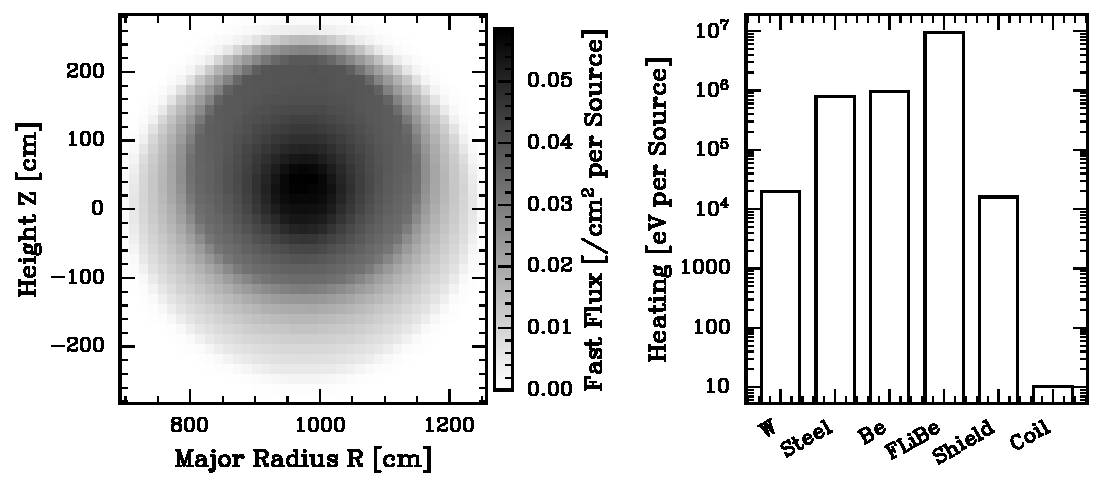
\includegraphics[width=\linewidth]{fig_conformal_flux.pdf}
\end{column}
\begin{column}{0.38\textwidth}
\footnotesize
\begin{itemize}
\item Native \texttt{StellaratorSource} transported through the full
      W/steel/Be/FLiBe/shield/coil DAGMC blanket, scattering on (device 59509).
\item FLiBe absorbs 84\% of the $1.1\times10^{7}$\,eV per source-neutron total heating.
\item Near-wall fast flux modulates perp $-10\%$ / parallel $+10\%$ vs unpolarized: the
      birth anisotropy survives to the flux tally, at reduced amplitude.
\end{itemize}
\end{column}
\end{columns}
\end{frame}

\begin{frame}[allowframebreaks]{Notes --- End-To-End: Transported Flux And Heating}
{\color{red}\footnotesize
\begin{itemize}
\item This is the full-fidelity result: the native \texttt{StellaratorSource} run \emph{end-to-end}
      through the complete W/steel/Be/FLiBe/shield/coil DAGMC blanket with \emph{scattering on},
      device 59509 (nfp 3, aspect 6.7), scaled $\times10$. The figure (\texttt{fig\_conformal\_flux.pdf})
      is a volumetric flux/heating map on the $(n_r,n_\phi,n_z)=(39,32,39)$ mesh.
\item \textbf{FLiBe = 84\% of heating.} Of the $1.1\times10^7$\,eV per source-neutron total heating,
      the 50\,cm FLiBe breeder absorbs 84\%. Expected: FLiBe is the thickest layer and the primary
      neutron-energy sink. Numbers from \texttt{PROVENANCE.md} (QA\_RESEARCH Q31).
\item \textbf{Near-wall fast flux: perp $-10\%$ / parallel $+10\%$ vs unpolarized.} This is the
      headline of the slide: the birth anisotropy \emph{survives transport to the flux tally}, but at
      reduced amplitude --- the volumetric echo of the surface steering. It shows polarization leaves a
      measurable footprint even with full scattering.
\item \textbf{The honest caveat to volunteer.} A volumetric mesh shows \emph{heating}, not
      \emph{inboard/outboard steering}: the near-field steering asymmetry is a \emph{surface} effect
      that a volumetric mesh cannot resolve. To see the in/out asymmetry properly you would need a
      first-wall surface-current tally (QA\_RESEARCH Q31). Say this before Ethan asks.
\item \textbf{Relation to the ``$\sim$3$\times$ dilution'' story.} Free-streaming, A-mode steers
      inboard $+40\%$/outboard $-20\%$; with the full blanket ON it drops to $+13.2\%$/$-9.2\%$ ---
      roughly a factor $\sim$3 of the first-flight lever survives. Physically, every scatter
      randomizes direction, so the wall load is uncollided (steered) + scattered (isotropized). This
      is the ``why you need transport'' result --- a free-streaming/analytic method overstates the
      benefit $\sim$3$\times$ (QA\_RESEARCH Q30). The $\pm10\%$ near-wall flux modulation here is the
      volumetric analog of that diluted surface lever.
\item HOW/WHERE: run via \texttt{run\_conformal.py}; the volumetric-flux device is 59509; results in
      \texttt{PROVENANCE.md}.
\item Likely follow-up (Ethan): ``does the $\pm10\%$ include the in/out asymmetry?'' --- crisp: no ---
      this mesh shows heating; the in/out steering is a surface-current effect, so the $\pm10\%$ is the
      polarization footprint on near-wall flux, not the steering asymmetry. Second likely: ``one
      device --- is that enough for the dilution claim?'' --- the $\sim$3$\times$ dilution rests on the
      box-torus Tier-5 blanket plus this 59509 conformal run; looping the scattering run over more
      QUASR devices is the acknowledged to-do (QA\_RESEARCH Q46).
\end{itemize}
}
\end{frame}

% ============================================================
\begin{frame}{Free-Streaming: Recovers Schwartz On Real Geometry}
\begin{columns}[c]
\begin{column}{0.55\textwidth}
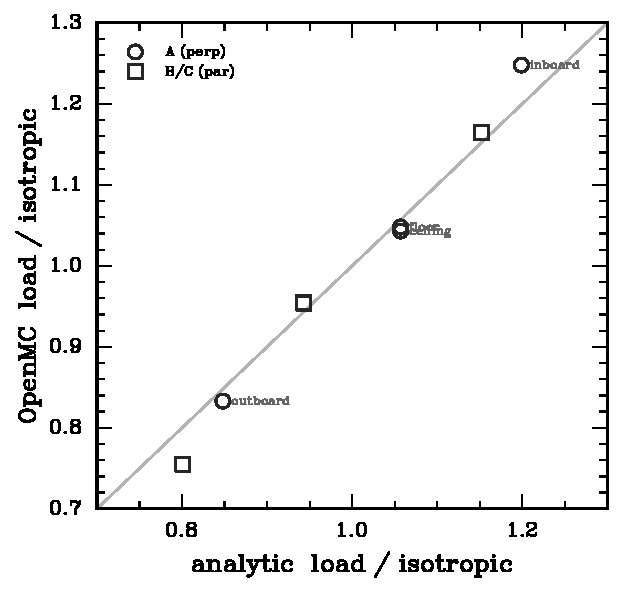
\includegraphics[width=\linewidth]{fig_quasr_validation.pdf}
\end{column}
\begin{column}{0.43\textwidth}
\footnotesize
\begin{itemize}
\item Axisymmetric limit (Schwartz recovery): A-mode midplane $+43\%$/$-22\%$ in the text,
      reproduced as $+39\%$/$-21\%$.
\item Independent cross-check: analytic point-patch vs ray-traced OpenMC on the conformal
      59509 wall agree 0.5--2.3\% by region, per-bin $r=0.91$.
\item Per-wall free-stream error: outboard 1.8\%, floor 0.8\%, ceiling 1.3\%,
      strongly-curved inboard 4.1\%.
\end{itemize}
\end{column}
\end{columns}
\end{frame}

\begin{frame}[allowframebreaks]{Notes --- Free-Streaming: Recovers Schwartz On Real Geometry}
{\color{red}\footnotesize
\begin{itemize}
\item This slide is the validation that the free-streaming source reproduces known analytic results
      --- both Schwartz's published axisymmetric numbers and an independent analytic point-patch on
      the real 3-D wall. The figure (\texttt{fig\_quasr\_validation.pdf}) overlays MC vs analytic NWL.
\item \textbf{Schwartz recovery (axisymmetric limit).} Running the free-streaming StellaratorSource on
      a square torus with $\bhat=\hat\varphi$ (\texttt{field\_model='toroidal'}), A-mode shifts the
      midplane wall load by $+43\%$ inboard / $-22\%$ outboard in Schwartz's text; we reproduce
      $+39\%$/$-21\%$. IMPORTANT: it is $+39$/$-21$ (MC) vs $+43$/$-22$ (analytic text) --- do not
      round to ``$+40$'' loosely; the small gap is meaningful (next bullet).
\item \textbf{Why not exact?} The $\sim$4-/1-point gap is the $\varepsilon_\text{eff}\approx0.43$
      shaping residual of \emph{this} device, not a sampler error. Both candidate causes were
      eliminated: the sampler is exact (A/iso $=(3/2)\sin^2\theta$ to 0.3\%/bin), and the analytic
      equals anarrima to $1.2\times10^{-12}$. On a low-shaping toy-QA patch ($\varepsilon_\text{eff}
      \approx0.08$) MC and analytic agree $\le1.8\%$ on \emph{all} walls; at $\varepsilon_\text{eff}
      \approx0.43$ the gap appears \emph{only} on the inboard wall (closest, most curved)
      (QA\_RESEARCH Q28).
\item \textbf{What causes the inboard residual specifically.} It is the \emph{point-patch
      approximation of the analytic}, not the MC. \texttt{bare\_cylinder\_demo.py} isolates it: a
      single shaped filament, analytic point-patch vs exact ray/surface intersection; the error grows
      $\approx s^2$ with shaping amplitude and is $\sim$3$\times$ larger on the convex inboard
      cylinder ($|\Delta|$ 0.002$\to$0.098 as $s$: 0$\to$1). The MC (sampler-exact, geometry-exact) is
      the reference; this is ``where MC is necessary'' (QA\_RESEARCH Q29).
\item \textbf{Independent cross-check on the real conformal wall.} \texttt{conformal\_freestream\_xcheck.py},
      device 59509: analytic point-patch vs ray-traced OpenMC StellaratorSource on the true 3-D
      conformal wall. Agree 0.5--2.3\% by region (inboard A/iso 1.6\%, B/iso 2.3\%; outboard
      0.5\%/0.6\%; global 0.9\%/1.2\%), per-bin correlation $r\approx0.91$. This validates the source
      free-streaming on \emph{real} geometry, not only the square torus (QA\_RESEARCH Q32).
\item \textbf{Per-wall error breakdown.} outboard 1.8\%, floor 0.8\%, ceiling 1.3\%, strongly-curved
      inboard 4.1\% --- the inboard is the worst because it is closest and most curved, consistent with
      the point-patch story above.
\item Likely follow-up (Ethan): ``is the inboard gap a bug in your sampler?'' --- crisp: no; the
      sampler is exact to 0.3\%/bin and the analytic equals anarrima to $10^{-12}$; the gap is the
      analytic point-patch losing accuracy on the high-curvature inboard wall, which is exactly why the
      MC is the reference there. Second likely: ``what is $\varepsilon_\text{eff}$?'' --- the helical
      excursion over the source-to-wall standoff (see the Predictors slide); 0.43 for 59509 puts it
      mid-regime where the analytic series is accurate but not perfect.
\end{itemize}
}
\end{frame}

% ============================================================
\begin{frame}{Free Streaming Poloidal NWL Maps}
\begin{columns}[c]
\begin{column}{0.6\textwidth}
\includegraphics[width=\linewidth]{nwl_maps.pdf}
\end{column}
\begin{column}{0.38\textwidth}
\footnotesize
\begin{itemize}
\item $(\theta,\phi)$ NWL on the conformal first wall for QUASR 886079, normalized to the
      mean.
\item Optimal polarization here is $a_2=+0.83$ (strongly parallel-leaning), lowering the
      peaking factor $1.78\to1.49$ (a 16\% reduction).
\item This is the free-streaming pattern; scattering dilutes the modulation.
\end{itemize}
\end{column}
\end{columns}
\end{frame}

\begin{frame}[allowframebreaks]{Notes --- Free Streaming Poloidal NWL Maps}
{\color{red}\footnotesize
\begin{itemize}
\item The figure (\texttt{nwl\_maps.pdf}) shows the neutron wall load as a 2-D map over
      $(\theta,\phi)$ --- poloidal angle $\times$ toroidal angle --- on the conformal first wall of
      QUASR device 886079, each panel normalized to its own mean so you compare \emph{shapes}. Bright
      = hot spot, dark = cold. Compare the unpolarized panel to the optimal-polarization panel to see
      the peak flatten.
\item \textbf{The headline number.} For 886079 the peaking-optimal polarization is $a_2=+0.83$
      (strongly parallel-leaning, i.e.\ emission biased along $\bhat$), which lowers the peaking
      factor (hot-spot/mean) from $1.78\to1.49$ --- a 16\% reduction. This is the \emph{best} device in
      the n=15 set; it is an outlier, not typical (median benefit is $\sim$4\%).
\item \textbf{What $a_2=+0.83$ means.} $a_2$ is the $P_2$ multipole coefficient: $a_2=+1$ is pure
      parallel (B/C shape), $a_2=-1$ pure perpendicular (A), $a_2=0$ unpolarized. $+0.83$ is close to
      fully parallel-leaning. The optimizer sweeps $a_2\in[-1,1]$ as $\text{unpol}+t(\text{par}-
      \text{unpol})$ and minimizes the peaking factor (QA\_RESEARCH Q8/Q34).
\item \textbf{Caveat on the slide.} ``This is the free-streaming pattern; scattering dilutes the
      modulation'' --- the 16\% is a free-streaming (first-flight) number; with a real blanket the
      lever shrinks $\sim$3$\times$ (the End-to-End slide's $\pm10\%$ near-wall echo). So do not
      present 16\% as a delivered reactor benefit.
\item HOW/WHERE: generated by \texttt{fig\_nwl\_maps.py}; the optimal-$a_2$ sweep is
      \texttt{predictor\_test.py:benefit()}.
\item Likely follow-up (Ethan): ``why parallel-optimal here when A-mode is the big-steering mode?'' ---
      crisp: A-mode (perp) pushes load \emph{inboard}; whether that helps or hurts peaking depends on
      where the device's hot spot already is. For 886079 the hot spot is such that a parallel
      (outboard-leaning) bias flattens it, so $a_2>0$ wins. The optimal $a_2$ flips sign across devices
      --- no single polarization helps everyone (next slides; QA\_RESEARCH Q34/Q36).
\end{itemize}
}
\end{frame}

% ============================================================
\begin{frame}{How Much Does Polarization Reduce Peaking?}
\begin{columns}[c]
\begin{column}{0.55\textwidth}
\includegraphics[width=\linewidth]{pf_hist.pdf}
\end{column}
\begin{column}{0.43\textwidth}
\footnotesize
\begin{itemize}
\item Ran the peaking-optimal polarization scan in the free-streaming limit for 15 QUASR
      reactor designs spanning shaping amplitude 0.16--1.00.
\item Optimal reduction is weak: 0--16\%, median $\approx4\%$; the 16\% case is an outlier.
\item The optimal $a_2$ itself flips sign across devices ($-0.83$ to $+1.0$): no single
      polarization helps every design.
\item For stellarators, polarization is not a strong peaking-factor lever.
\end{itemize}
\end{column}
\end{columns}
\end{frame}

\begin{frame}[allowframebreaks]{Notes --- How Much Does Polarization Reduce Peaking?}
{\color{red}\footnotesize
\begin{itemize}
\item This is the honest ``how big is the effect'' slide. The figure (\texttt{pf\_hist.pdf}) is a
      histogram of the optimal peaking-factor reduction $Y=(PF_\text{unpol}-\min_{a_2}PF)/
      PF_\text{unpol}$ across the 15 free-streaming devices. Read it as: most bars pile up at small
      benefit ($\sim$0--5\%), with one outlier out at 16\%.
\item \textbf{The 15 devices.} Peaking-optimal polarization scan, free-streaming limit, 15 QUASR
      reactor designs spanning shaping amplitude 0.16--1.00 (near-round to strongly shaped), aspect
      ratio 3.3--24, nfp 2--5, mostly quasi-axisymmetric. Provenance: a stratified mine of the 371,701-
      device QUASR catalogue $\to$ VMEC batch (30 devices, 22 converged) $\to$ conformal batch $\to$ 15
      usable maps, plus the 5 originals (QA\_RESEARCH A4/Q34).
\item \textbf{The result: weak.} Optimal reduction is 0--16\%, median $\approx$4\%; the 16\% case
      (886079, previous slide) is an outlier. So on the previous slide's device you saw the \emph{best}
      case; typical is much smaller.
\item \textbf{The optimal $a_2$ flips sign ($-0.83$ to $+1.0$).} No single polarization setting helps
      every design --- some want perpendicular ($a_2<0$), most want parallel ($a_2>0$). This kills any
      ``just polarize the fuel this one way'' universal recipe.
\item \textbf{Take-home.} For stellarators, polarization is \emph{not} a strong peaking-factor lever.
      This is a genuine (honest, non-cherry-picked) null-ish result and one of the paper's points ---
      SPF is a local actuator, not a global flattener.
\item \textbf{Why it is weak (mechanism).} Peaking is dominated by a narrow near-field grazing spike
      (0.3--2.8\% of wall area) that the $P_2$ angular lever \emph{cannot} move; SPF only steers the
      broad, low-harmonic in/out asymmetry (the $\pm$22--43\% lever). So benefit tracks available
      \emph{headroom}, not shaping. Free-streaming line-of-sight integration is a spatial low-pass
      filter $T(N)\sim e^{-Na/R_0}$, so the wall structurally cannot resolve high-harmonic shaping
      (QA\_RESEARCH Q35).
\item Likely follow-up (Ethan): ``is 16\% real or noise?'' --- crisp: it is a real free-streaming
      optimum for 886079, but (a) it is an outlier and (b) scattering would dilute it $\sim$3$\times$,
      so the delivered reactor benefit is small. Second likely: ``why does the optimal $a_2$ flip
      sign?'' --- because it depends on where each device's hot spot sits relative to the in/out
      asymmetry; perp pushes load inboard, parallel outboard, and the beneficial direction is
      device-specific.
\end{itemize}
}
\end{frame}

% ============================================================
\begin{frame}{Predictors Of Steerability}
\footnotesize
Three metrics we test as forecasts of the free-streaming steering benefit:
\begin{itemize}
\item PF$_\mathrm{geo}$ (geometry-only headroom): a transport-free peaking factor from an
      isotropic $1/r^2$ flux proxy $G(\mathbf{w})=\sum_v |\sqrt{g}|_v/|\mathbf{w}-\mathbf{r}_v|^2$
      over source voxels, $\mathrm{PF}_\mathrm{geo}=\max G/\langle G\rangle_A$. High means the
      wall load is geometrically peaked before any physics.
\item Nematic $Q$ (pure plasma shape): $Q=|\langle e^{2i\psi}\rangle|$ over the LCFS
      outward-normal angles $\psi=\arctan2(n_Z,n_R)$. The nematic order of the wall-normal
      director field --- $0$ = orientations isotropic, $1$ = fully aligned.
\item $\varepsilon_\mathrm{eff}$ (helical standoff, my parameter): the non-axisymmetric
      boundary excursion relative to the source-to-wall standoff --- a property of the
      boundary geometry, not $|B|$ quasi-symmetry. Small ($\lesssim0.15$): the analytic
      $P_2$ series is second-order accurate; large ($\gtrsim2$): the series breaks down and
      needs hybrid quadrature. Device 59509: $\varepsilon_\mathrm{eff}\approx0.43$.
\end{itemize}
\end{frame}

\begin{frame}[allowframebreaks]{Notes --- Predictors Of Steerability}
{\color{red}\footnotesize
\begin{itemize}
\item This slide defines the three metrics we test as \emph{forecasts} of the free-streaming steering
      benefit --- can we predict, cheaply, which devices SPF will help, without running transport?
\item \textbf{PF$_\text{geo}$ --- geometry-only headroom (the best predictor).} Formula
      (\texttt{predictor\_test.py:geometry()}): a transport-free isotropic $1/r^2$ flux proxy
      $G(\mathbf{w})=\sum_v w_v/|\mathbf{w}-\mathbf{r}_v|^2$ over source voxels $\mathbf{r}_v$ (the
      fluxmap nodes) with per-voxel weight $w_v=|\sqrt{g}|_v/\sum|\sqrt{g}|$, evaluated at wall points
      $\mathbf{w}$ (conformal wall = LCFS offset outward by $0.30a$). Then $PF_\text{geo}=\max_k G(w_k)/
      \sum_k G(w_k)\,dA_k$ = max over area-weighted-mean. PLAIN ENGLISH: the wall load a point
      \emph{isotropic} source cloud would deposit using only inverse-square geometry --- no scattering,
      no angular physics. Its peaking factor is the ``headroom'' SPF has to flatten, computed in
      milliseconds. It is the best single predictor (Spearman $\rho=+0.525$) but only borderline at
      n=15 (QA\_RESEARCH A1/Q34).
\item \textbf{Nematic $Q$ --- pure plasma shape.} $Q=|\langle e^{2i\psi}\rangle|$ where
      $\psi=\arctan2(n_Z,n_R)$ is the angle of each LCFS \emph{outward normal} in the (R,Z) plane. The
      factor $2\psi$ (not $\psi$) makes it orientation-blind --- a director is a headless axis (period
      $\pi$), so $n$ and $-n$ count the same, as for liquid-crystal directors. $Q=0$ = normals point
      every which way (strongly/asymmetrically shaped); $Q=1$ = all normals aligned (slab/ellipse-like).
      It is a \emph{pure shape} metric --- LCFS only, no wall, no transport. Verdict: does NOT robustly
      forecast steering ($\rho=+0.396$, not significant) (QA\_RESEARCH A2/Q34).
\item \textbf{$\varepsilon_\text{eff}$ --- helical standoff (my coined parameter).} Definition:
      $\varepsilon_\text{eff}\sim \max_\phi\sqrt{dR^2+dZ^2}/\min_\phi|\Delta_0|$ = (non-axisymmetric
      boundary excursion) / (smallest source-to-wall standoff). It is a property of the \emph{boundary
      geometry}, NOT of $|B|$ quasi-symmetry (a QA device need not be geometrically axisymmetric ---
      say this, it is a subtle point Ethan will probe). It controls the analytic $P_2$ series
      truncation error, which scales as $\varepsilon_\text{eff}^{p+1}$ at order $p$
      (QA\_RESEARCH A3).
\item \textbf{The $\varepsilon_\text{eff}$ regime thresholds (get these RIGHT).} $\varepsilon_\text{eff}
      \lesssim 0.15$: the second-order series is already $\le$1.5\% accurate (Schwartz's uniform-NWL
      residual level) --- the QA regime where $g^0+g^1+g^2$ suffices. $\varepsilon_\text{eff}<1$: series
      still convergent (needs higher orders as it grows). $\varepsilon_\text{eff}\gtrsim 2$: the series
      \emph{breaks down} (characteristic spurious double-peak in the inboard valley), must fall back to
      differentiable hybrid quadrature. Device 59509: $\varepsilon_\text{eff}\approx 0.43$ (mid-regime:
      accurate but not perfect, which is why its Schwartz recovery is $+39/-21$ not exactly $+43/-22$).
      NOTE: the correct thresholds are $\lesssim 0.15$ (2nd-order accurate) and $\gtrsim 2$ (breakdown)
      --- there is NO ``$\sim 1/2$'' threshold; do not state one (QA\_RESEARCH A3, explicit).
\item Reference $\varepsilon_\text{eff}$ values for published QAs at a tight wall: precise\_QA/reactor\_QA
      2.3 (MC-only), ESTELL 1.0, NCSX 1.3, ARIES-CS 1.6, WISTELL-A 1.6; toy-QA-low patch 0.08
      (QA\_RESEARCH A3).
\item Likely follow-up (Ethan): ``isn't $\varepsilon_\text{eff}$ just quasi-symmetry error?'' --- crisp:
      no --- it is purely geometric (boundary excursion / standoff); a $|B|$-quasi-symmetric device can
      still be geometrically very non-axisymmetric, so $\varepsilon_\text{eff}$ and QS error are
      distinct. Second likely: ``why is PF$_\text{geo}$ the best predictor?'' --- because SPF can only
      flatten peaking that geometry already bakes in; PF$_\text{geo}$ measures exactly that headroom,
      and the benefit tracks headroom rather than plasma shape.
\end{itemize}
}
\end{frame}

\begin{frame}{When Does Polarization Help? (n=15)}
\begin{columns}[c]
\begin{column}{0.55\textwidth}
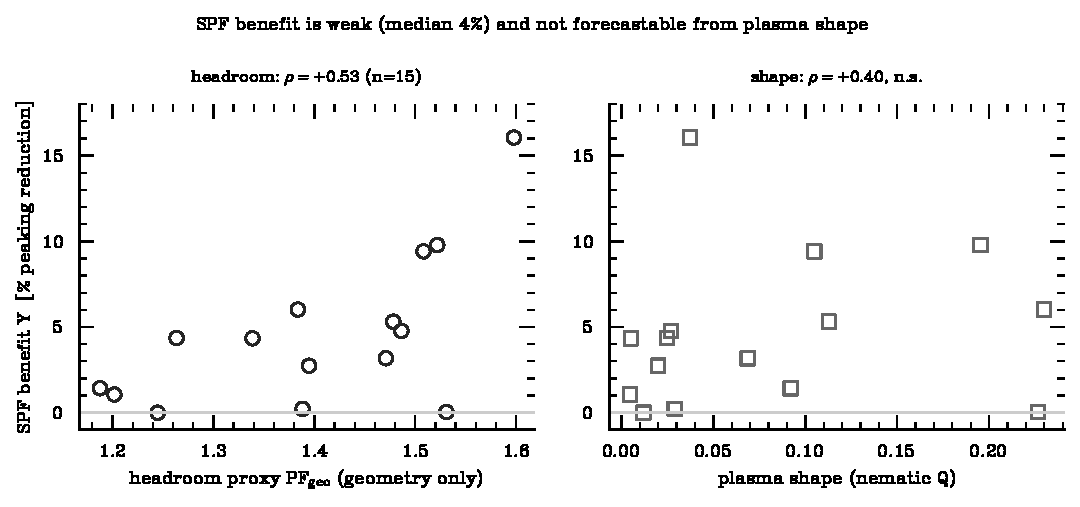
\includegraphics[width=\linewidth]{fig_predictor.pdf}
\end{column}
\begin{column}{0.43\textwidth}
\footnotesize
\begin{itemize}
\item Peaking-factor benefit across 15 conformal-wall QUASR devices is weak everywhere:
      0--16\%, median 4\%.
\item Best predictor is the transport-free headroom PF$_\mathrm{geo}$ ($\rho=+0.53$,
      borderline at $n=15$).
\item Plasma shape (nematic $Q$, $\rho=+0.40$) does not robustly forecast the benefit.
\item Devices drawn from the QUASR database, stratified by symmetry class and field
      period; 30 VMEC solves gave 15 usable conformal maps (aspect ratio 3.3--24, mostly
      quasi-axisymmetric).
\end{itemize}
\end{column}
\end{columns}
\end{frame}

\begin{frame}[allowframebreaks]{Notes --- When Does Polarization Help? (n=15)}
{\color{red}\footnotesize
\begin{itemize}
\item This slide is the predictor \emph{result} --- the scatter of benefit vs each metric. The figure
      (\texttt{fig\_predictor.pdf}) plots the SPF benefit $Y$ against the predictors with the Spearman
      correlations annotated. Look for whether the points trend (they barely do).
\item \textbf{The n=15 numbers to state (these are the current, non-stale ones).} Benefit is weak
      everywhere: 0--16\%, median 4\%. Best predictor is transport-free headroom PF$_\text{geo}$ with
      Spearman $\rho=+0.53$ (borderline at n=15). Plasma shape (nematic $Q$) does NOT robustly forecast:
      $\rho=+0.40$, not significant. (\texttt{shaping\_amp} is $\rho=-0.186$, also n.s.)
      (QA\_RESEARCH Q34.)
\item \textbf{IMPORTANT --- do not quote the stale n=5 numbers.} An earlier n=5 run showed
      PF$_\text{geo}$ $\rho=+0.90$; that strong correlation \emph{regressed to noise} at n=15 (a
      properly-powered null). Always cite the n=15 values (PF$_\text{geo}$ $\rho=+0.525$, nematic $Q$
      $\rho=+0.396$), not the old +0.90. If Ethan remembers the +0.90, explain it was underpowered.
\item \textbf{Device provenance (for the ``is the sample fair?'' question).} Devices drawn from the
      371,701-device QUASR catalogue, stratified by symmetry class (QA/QH), nfp, quasisymmetry-error
      quintile, and aspect ratio (seed 20260707), to \emph{span} not cluster. 30 VMEC solves $\to$ 22
      converged $\to$ 15 usable conformal maps, plus the 5 originals. Span: aspect ratio 3.33--24, nfp
      2--5, mostly quasi-axisymmetric ($\sim$13 QA + 2 QH; QH under-represented because fixed-boundary
      VMEC rejects strongly-shaped QH). Shaping amplitude 0.16--1.00 (QA\_RESEARCH A4).
\item \textbf{The interesting outlier: 803097.} Peaked (PF$_\text{unpol}$=1.40) but \emph{unsteerable}
      ($Y=0.014$, $\sim$10$\times$ below the rest) and the \emph{only} perp-optimal device ($a_2^\text{opt}=
      -0.83$). PF$_\text{geo}$ flags it as \emph{low} peaking (1.19), so its transport peaking comes from
      an anisotropic near-field structure the isotropic proxy cannot see --- both perp-favorable and
      steering-resistant. This is ``when SPF cannot help'' (QA\_RESEARCH Q36).
\item \textbf{The honest caveat on the mechanism.} The claim ``plasma shape can't predict steering'' is
      supported by the n=15 null but not independently proven --- the low-pass-filter argument
      ($T(N)\sim e^{-Na/R_0}$) is directly validated only for the \emph{ripple}, and \texttt{shaping\_amp}
      did not cleanly decouple. State it as supported-not-proven (QA\_RESEARCH Q35).
\item Likely follow-up (Ethan): ``$\rho=+0.53$ at n=15 --- is that significant?'' --- crisp: borderline;
      it is the best of the three but I would not over-claim it; the honest statement is that benefit
      tracks geometric headroom weakly and plasma shape not at all, and n=15 is underpowered for a firm
      p-value. Second likely: ``why did the n=5 correlation collapse?'' --- underpowered; five points can
      show $\rho=0.9$ by chance, and the properly-sampled n=15 set regressed it to noise.
\end{itemize}
}
\end{frame}

% ============================================================
\begin{frame}{Summary}
Done and verified
\begin{itemize}\footnotesize
\item Native polarized \texttt{Source} plus a 3-D \texttt{StellaratorSource}; the sampler is
      exact ($\chi^2$, KS, moments, $a_2$-linearity).
\item Free-streaming cross-validated against an independent analytic point-patch on real
      QUASR geometry.
\item End-to-end conformal blanket transport with scattering.
\end{itemize}
Limitations
\begin{itemize}\footnotesize
\item Monoenergetic 14.06\,MeV (the \texttt{TokamakSource} energy handling is richer).
\item Constant/toroidal or gridded $\bhat$ only; no depolarization; convex-ish walls.
\item Steering is a source/free-stream effect; scattering dilutes it $\sim3\times$, and the
      peaking-factor benefit is weak for stellarators.
\end{itemize}
\end{frame}

\begin{frame}[allowframebreaks]{Notes --- Summary}
{\color{red}\footnotesize
\begin{itemize}
\item Closing slide: three ``done'' claims and three honest limitations. Each maps to a prior slide.
\item \textbf{Done 1: native polarized Source + 3-D StellaratorSource, sampler exact.} ``Exact'' is
      backed by four independent Tier-1 gates: $\chi^2$ on $\cos\theta$ marginals, inverse-CDF-vs-
      rejection KS, emission moments $\langle(\mathbf{u}\cdot\bhat)^2\rangle$ matching analytic to
      $10^{-3}$, and the $a_2$-linearity identity. (Verification slide.)
\item \textbf{Done 2: free-streaming cross-validated against an independent analytic point-patch on
      real QUASR geometry.} 0.5--2.3\% by region, per-bin $r\approx0.91$, on the conformal 59509 wall
      --- plus the Schwartz $+43/-22 \to +39/-21$ recovery on the box torus. (Free-Streaming slides.)
\item \textbf{Done 3: end-to-end conformal blanket transport with scattering.} Full W/steel/Be/FLiBe/
      shield/coil DAGMC, FLiBe 84\% of heating, near-wall flux $\pm10\%$ modulation. (End-to-End slide.)
\item \textbf{Limitation 1: monoenergetic 14.06\,MeV.} TokamakSource carries richer per-$r$ Ballabio
      spectra; ours is one distribution for all $\rho$. Energy is decoupled from the polarized angular
      physics, so it does not affect the steering verification, and per-$r$ spectra are a drop-in (XML
      already loops \texttt{<energy>}) (QA\_RESEARCH Q20/Q42).
\item \textbf{Limitation 2: field/wall restrictions.} Constant/toroidal or gridded $\bhat$ only; no
      depolarization physics (once born, neutrons transport unpolarized --- standard cross sections,
      same scope as Bae); convex-ish walls (the analytic oracle assumes a single visible arc; the MC
      ray-traces the true wall with no such restriction) (QA\_RESEARCH Q43/Q44).
\item \textbf{Limitation 3: the headline honest result.} Steering is a source/free-stream effect;
      scattering dilutes it $\sim$3$\times$; and the peaking-factor benefit is weak for stellarators
      (0--16\%, median 4\%). SPF is a local actuator, not a global flattener --- and quantifying the
      $\sim$3$\times$ dilution is precisely why you need transport rather than the analytic
      (QA\_RESEARCH Q30/Q45).
\item Likely follow-up (Ethan): ``what do you want from me?'' --- crisp: co-author sign-off on the
      later sections; a sanity check on the TokamakSource upstreaming path for the \texttt{<polarization>}
      hook; and a view on whether \texttt{spf\_fluxmap\_v1} vs reading OpenMC's HDF5 mesh/field infra is
      acceptable for an eventual upstream (QA\_RESEARCH Q50).
\end{itemize}
}
\end{frame}

\begin{frame}{Backup: One-Glance Number Table}
\scriptsize
\begin{tabular}{@{}lccccc@{}}
\toprule
mode & $\eta$ & rate & center-stack & inboard NWL$^\ast$ & outboard NWL$^\ast$ \\
\midrule
unpolarized & 0.667 & 1.00 & 1.00 & --- & --- \\
A (perp) & 1.000 & 1.50 & 1.70 & $+40\%\!\to\!+13\%$ & $-20\%\!\to\!-9\%$ \\
B (par) & 0.667 & 1.00 & 0.85 & $-40\%\!\to\!-15\%$ & $+19\%\!\to\!+9\%$ \\
C & 0.333 & 0.50 & 0.42 & (B shape) & (B shape) \\
\bottomrule
\end{tabular}
\vfill
\footnotesize
$^\ast$ Free-Streaming $\to$ full transport. Directional efficiency of the pitched 3-D
field vs pure axisymmetric $\hat\varphi$: $\eta_{\text{dir}}=0.89$. Schwartz recovery
(A midplane): analytic $+43/-22\%$, OpenMC $+39/-21\%$.
\end{frame}

\begin{frame}[allowframebreaks]{Notes --- Backup: One-Glance Number Table}
{\color{red}\footnotesize
\begin{itemize}
\item This backup table is the one-glance cheat sheet tying rate and steering together per mode. Read
      each row as: mode, total-rate factor $\eta$, relative fusion rate, center-stack load, and the
      inboard/outboard NWL change shown as free-streaming $\to$ full-transport.
\item \textbf{$\eta$ column (from the physics slide).} unpolarized 0.667, A 1.000, B 0.667, C 0.333 ---
      these are $a+\tfrac23 b+\tfrac13 c$ at the four corners. ``rate'' normalizes $\eta$ to the
      unpolarized value: A = 1.50 ($+50\%$), B = 1.00 (same), C = 0.50 (half).
\item \textbf{center-stack column.} Relative inboard (center-stack) load: A pushes load inboard (1.70),
      B pulls it outboard (0.85), C same shape as B at half rate (0.42). Unpolarized = 1.00 reference.
\item \textbf{inboard/outboard NWL, free-streaming $\to$ transport.} A: inboard $+40\%\to+13\%$,
      outboard $-20\%\to-9\%$; B mirrors it $-40\%\to-15\%$ inboard, $+19\%\to+9\%$ outboard; C shares
      B's shape. The arrow is the $\sim$3$\times$ scattering dilution --- the free-streaming lever on
      the left, what survives full blanket transport on the right (QA\_RESEARCH Q30).
\item \textbf{The two footnote numbers.} (1) $\eta_\text{dir}=0.89$: directional efficiency of the real
      pitched 3-D field vs a pure axisymmetric $\hat\varphi$ --- parallel mode reduces the inboard load
      2.2\% with the 3-D QA field vs 2.4\% with pure toroidal, so $\eta_\text{dir}=2.2/2.4\approx0.89$;
      the pitched field tilts $\bhat$ off $\hat\varphi$, costing $\sim$11\% of the ideal lever
      (QA\_RESEARCH Q33). (2) Schwartz recovery: analytic $+43/-22\%$ vs OpenMC $+39/-21\%$ --- the
      $\varepsilon_\text{eff}\approx0.43$ residual, not a sampler error (QA\_RESEARCH Q28).
\item \textbf{The rate-vs-steering trade (Tier 7 context).} B is the ``sweet spot'': A gives the biggest
      steering ($+70\%$ center-stack) but needs full alignment ($\eta=1$); C halves the rate; B keeps the
      non-polarized rate ($\eta=\tfrac23$, fusion\_rate 1.00) \emph{while still steering} (center-stack
      0.85, outboard 1.09). TBR/neutron is nearly mode-flat ($\sim$1.15) (QA\_RESEARCH Q37).
\item Likely follow-up (Ethan): ``if A steers most but halves nothing, why not always run A?'' --- crisp:
      A requires full spin alignment (hard to achieve/maintain) and is perpendicular-steering only; B
      preserves the unpolarized fusion rate while still giving a useful directional lever, so B is the
      practical rate-preserving choice. Second likely: ``why $\eta_\text{dir}=0.89$ not 1?'' --- the real
      3-D field is pitched, so $\bhat$ is not exactly $\hat\varphi$; the tilt costs $\sim$11\% of the
      ideal axisymmetric steering lever.
\end{itemize}
}
\end{frame}

\end{document}
